%Version 3.1 December 2024
%%%%%%%%%%%%%%%%%%%%%%%%%%%%%%%%%%%%%%%%%%%%%%%%%%%%%%%%%%%%%%%%%%%%%%%
%% MambaATM, reworked manuscript.
%%
%% This file replaces the version that was reviewed. Two things changed.
%%
%% 1. The architecture description now matches the implementation. The submitted text described
%%    attention guiding the state update of the state-space branch. The submitted code computed a
%%    sigmoid gate over the two branch outputs and mixed them, which is a gated convex combination.
%%    Section 4 describes the gate, and the guided modulation is implemented and measured as a
%%    separate variant, so the difference between the claim and the artefact is now a result.
%%
%% 2. The experiments were rebuilt on a panel that can be verified. Every number in the text is
%%    emitted by a script from the same result files that produce the tables.
%%
%% Every quantity quoted in prose is a macro from numbers.tex, generated by emit_numbers.py.
%%%%%%%%%%%%%%%%%%%%%%%%%%%%%%%%%%%%%%%%%%%%%%%%%%%%%%%%%%%%%%%%%%%%%%%

\PassOptionsToPackage{hidelinks}{hyperref}
\documentclass[pdflatex,sn-mathphys-ay]{sn-jnl}

%%%% Standard Packages
\usepackage{graphicx}%
\usepackage{multirow}%
\usepackage{amsmath,amssymb,amsfonts}%
\usepackage{amsthm}%
\usepackage{mathrsfs}%
\usepackage{amsbsy,latexsym}%
\usepackage{cancel}%
\usepackage[title]{appendix}%
\usepackage{xcolor}%
\usepackage{textcomp}%
\usepackage{array}%
\usepackage{tabularx}%
\usepackage{colortbl}%
\usepackage{makecell}%
\usepackage{booktabs}%
\usepackage{float}%
\usepackage{subcaption}%
\usepackage{algorithm}%
\usepackage{algorithmicx}%
\usepackage{algpseudocode}%
\usepackage{url}%
\usepackage{cleveref}%
\crefname{figure}{Fig.}{Figs.}%
\crefname{table}{Table}{Tables}%
\crefname{equation}{Eq.}{Eqs.}%
%%%%

\theoremstyle{thmstyleone}%
\newtheorem{Assumption}{Assumption}[section]%
\newtheorem{theorem}{Theorem}%
\newtheorem{proposition}[theorem]{Proposition}%
\newtheorem{Lemma}{Lemma}[section]%
\theoremstyle{thmstyletwo}%
\newtheorem{example}{Example}%
\newtheorem{remark}{Remark}%
\theoremstyle{thmstyletwo}%
\newtheorem{definition}{Definition}%

% generated by emit_numbers.py and make_paper_assets.py, merged -- do not edit
\newcommand{\nStocks}{232}
\newcommand{\nModels}{10}
\newcommand{\nFolds}{5}
\newcommand{\seqLen}{60}
\newcommand{\nEpochs}{30}
\newcommand{\seedUsed}{0}
\newcommand{\runMinutes}{144}
\newcommand{\nPanelRows}{610\,988}
\newcommand{\nDays}{2\,673}
\newcommand{\nStockDays}{587\,751}
\newcommand{\nSuspDays}{22\,798}
\newcommand{\pctSusp}{3.7\%}
\newcommand{\nNoPrevRows}{232}
\newcommand{\nNoLabelRows}{232}
\newcommand{\nOverlapRows}{25}
\newcommand{\nRemovedRows}{23\,237}
\newcommand{\firstDate}{2015-01-06}
\newcommand{\lastDate}{2025-12-31}
\newcommand{\minRows}{1124}
\newcommand{\medRows}{2596}
\newcommand{\maxRows}{2671}
\newcommand{\maxRankCorr}{0.100}
\newcommand{\medRankCorr}{0.043}
\newcommand{\acfMean}{+0.080}
\newcommand{\acfMin}{-0.034}
\newcommand{\acfMax}{+0.228}
\newcommand{\nFeatures}{8}
\newcommand{\accMaj}{0.528}
\newcommand{\accLong}{0.473}
\newcommand{\retBH}{+67.9\%}
\newcommand{\shBH}{+0.30}
\newcommand{\ddBH}{65.0\%}
\newcommand{\medRetBH}{+44.4\%}
\newcommand{\accProp}{0.516}
\newcommand{\accPropSd}{0.021}
\newcommand{\precProp}{0.476}
\newcommand{\recallProp}{0.324}
\newcommand{\icProp}{+0.0093}
\newcommand{\shProp}{+0.15}
\newcommand{\ddProp}{42.6\%}
\newcommand{\retProp}{+29.9\%}
\newcommand{\retPropSd}{104.3\%}
\newcommand{\turnProp}{0.076}
\newcommand{\beatMajProp}{24\%}
\newcommand{\beatBHProp}{34\%}
\newcommand{\accMLP}{0.516}
\newcommand{\accMLPSd}{0.019}
\newcommand{\accLSTM}{0.519}
\newcommand{\accLSTMSd}{0.021}
\newcommand{\accAtt}{0.518}
\newcommand{\accAttSd}{0.019}
\newcommand{\accDLinear}{0.521}
\newcommand{\accDLinearSd}{0.022}
\newcommand{\accPatch}{0.514}
\newcommand{\accPatchSd}{0.022}
\newcommand{\accITrans}{0.507}
\newcommand{\accITransSd}{0.019}
\newcommand{\accTimes}{0.513}
\newcommand{\accTimesSd}{0.019}
\newcommand{\accSSM}{0.514}
\newcommand{\accSSMSd}{0.022}
\newcommand{\accGuided}{0.517}
\newcommand{\accGuidedSd}{0.021}
\newcommand{\accBest}{0.521}
\newcommand{\accBestName}{DLinear}
\newcommand{\accSecond}{0.521}
\newcommand{\accSecondName}{DLinear}
\newcommand{\accWorst}{0.507}
\newcommand{\shBest}{+0.18}
\newcommand{\shBestName}{attention with a causal convolution}
\newcommand{\retBest}{+19.5\%}
\newcommand{\rangeAcc}{1.4}
\newcommand{\fOneBest}{0.409}
\newcommand{\fOneBestName}{iTransformer}
\newcommand{\beatMajBest}{26.3\%}
\newcommand{\beatMajBestName}{attention with a causal convolution}
\newcommand{\accGuidedMinusPlain}{+0.10}
\newcommand{\shGuided}{+0.12}
\newcommand{\shGuidedMinusPlain}{-0.03}
\newcommand{\paramProposed}{23\,242}
\newcommand{\paramGuided}{25\,452}
\newcommand{\paramSSM}{1\,057}
\newcommand{\paramPatch}{101\,953}
\newcommand{\paramMLP}{69\,889}
\newcommand{\paramDLinear}{147}
\newcommand{\turnBest}{0.141}
\newcommand{\turnBestName}{the selective SSM branch alone}
\newcommand{\secProposed}{27}
\newcommand{\secPatch}{25}
\newcommand{\secMLP}{5}
\newcommand{\secLSTM}{14}
\newcommand{\secAtt}{9}
\newcommand{\portDays}{2117}
\newcommand{\portBreadth}{163}
\newcommand{\portAnnBH}{-1.4\%}
\newcommand{\portShBH}{+0.07}
\newcommand{\portDDBH}{63.7\%}
\newcommand{\portTotalBH}{-11\%}
\newcommand{\portAnnProp}{-1.0\%}
\newcommand{\portShProp}{+0.09}
\newcommand{\portDDProp}{64.5\%}
\newcommand{\portTurnProp}{0.00}
\newcommand{\portAnnPropLow}{-1.0\%}
\newcommand{\portShPropLow}{+0.09}
\newcommand{\portDDPropLow}{64.4\%}
\newcommand{\portTurnPropLow}{0.00}
\newcommand{\portAnnPropHigh}{-1.0\%}
\newcommand{\portShPropHigh}{+0.08}
\newcommand{\portDDPropHigh}{64.5\%}
\newcommand{\portTurnPropHigh}{0.00}
\newcommand{\portAnnPropZero}{-0.9\%}
\newcommand{\portShPropZero}{+0.09}
\newcommand{\portDDPropZero}{64.4\%}
\newcommand{\portTurnPropZero}{0.00}
\newcommand{\portBestName}{DLinear}
\newcommand{\portAnnBest}{+2.9\%}
\newcommand{\portShBest}{+0.24}
\newcommand{\portDDBest}{44.4\%}
\newcommand{\nPortBeatBH}{10}
\newcommand{\nPortProfit}{5}
\newcommand{\portProfitNames}{DLinear, LSTM, PatchTST, TimesNet, the selective SSM branch alone}
\newcommand{\friedmanAcc}{152.1}
\newcommand{\friedmanAccP}{3.2e-28}
\newcommand{\friedmanSh}{29.2}
\newcommand{\friedmanShP}{0.00059}
\newcommand{\rankPropAcc}{5.32}
\newcommand{\rankPropSh}{5.27}
\newcommand{\rankBestAccName}{DLinear}
\newcommand{\nSignificantVsProp}{2}
\newcommand{\nCompared}{9}
\newcommand{\pMinVsProp}{9.86e-10}
\newcommand{\accBeatsName}{iTransformer}
\newcommand{\accLosesToName}{DLinear}
\newcommand{\nAccLead}{-0.54}
\newcommand{\nGateGain}{-0.17}
\newcommand{\secRatio}{5.2}
\newcommand{\shPropZero}{+0.09}
\newcommand{\accTMin}{0.516}
\newcommand{\accTMax}{0.516}
\newcommand{\accMajTMin}{0.525}
\newcommand{\accMajTMax}{0.526}
\newcommand{\accSeedSd}{0.30}
% ---- from the cross-sectional study ----
\newcommand{\nRows}{610\,988}
\newcommand{\nFactors}{29}
\newcommand{\nDates}{1{,}604}
\newcommand{\nStocksUsed}{231}
\newcommand{\nTestRows}{362{,}296}
\newcommand{\ccMean}{+0.0537}
\newcommand{\onMean}{-0.0597}
\newcommand{\idMean}{+0.1168}
\newcommand{\ccSd}{2.811}
\newcommand{\onSd}{1.379}
\newcommand{\idSd}{2.588}
\newcommand{\dilutionRatio}{2.04}
\newcommand{\icCcProp}{0.0671}
\newcommand{\tCcProp}{20.8}
\newcommand{\icOnProp}{0.1241}
\newcommand{\tOnProp}{45.3}
\newcommand{\icIdProp}{0.0158}
\newcommand{\identityProp}{0.0609}
\newcommand{\winsorProp}{0.1239}
\newcommand{\liquidProp}{0.1558}
\newcommand{\withinProp}{0.1377}
\newcommand{\icCcGuided}{0.0721}
\newcommand{\tCcGuided}{21.7}
\newcommand{\icOnGuided}{0.1369}
\newcommand{\tOnGuided}{48.6}
\newcommand{\icIdGuided}{0.0161}
\newcommand{\identityGuided}{0.0672}
\newcommand{\winsorGuided}{0.1368}
\newcommand{\liquidGuided}{0.1639}
\newcommand{\withinGuided}{0.1443}
\newcommand{\icCcTurn}{0.0678}
\newcommand{\tCcTurn}{14.4}
\newcommand{\icOnTurn}{0.1440}
\newcommand{\tOnTurn}{41.3}
\newcommand{\icIdTurn}{0.0159}
\newcommand{\identityTurn}{0.0706}
\newcommand{\winsorTurn}{0.1438}
\newcommand{\liquidTurn}{0.1834}
\newcommand{\withinTurn}{0.1469}
\newcommand{\liquidMedianAdvM}{90}
\newcommand{\pNearlyAllParticipation}{38}
\newcommand{\pNearlyAllParticipationFull}{38}
\newcommand{\residGuided}{0.0041}
\newcommand{\tResidGuided}{2.3}
\newcommand{\residProp}{0.0047}
\newcommand{\tResidProp}{2.7}
\newcommand{\rSquaredLo}{0.69}
\newcommand{\rSquaredHi}{0.89}
\newcommand{\bestFactorResid}{0.0242}
\newcommand{\bestFactorName}{Intraday range (20 days)}
\newcommand{\bestFactorT}{14.2}
\newcommand{\residCcBest}{0.0102}
\newcommand{\residCcBestName}{MambaATM (gated)}
\newcommand{\grossWk}{+77.6}
\newcommand{\onWkW}{+126.5}
\newcommand{\idWk}{-50.1}
\newcommand{\openWk}{-10.0}
\newcommand{\feeWk}{12.4}
\newcommand{\impactWk}{28.5}
\newcommand{\borrowWk}{8.0}
\newcommand{\netWk}{+28.7}
\newcommand{\grossDay}{+115.3}
\newcommand{\impactDay}{169.4}
\newcommand{\netDay}{-102.4}
\newcommand{\onDay}{+164.2}
\newcommand{\idDay}{-49.9}
\newcommand{\combName}{0.25 MambaATM (guided) + 0.75 cheap factors}
\newcommand{\combNet}{+33.9}
\newcommand{\combGross}{+79.1}
\newcommand{\combCap}{525.99}
\newcommand{\combIcCc}{0.0868}
\newcommand{\combIcOn}{0.1593}
\newcommand{\combTOn}{43.1}
\newcommand{\facNet}{+27.1}
\newcommand{\facCap}{409.11}
\newcommand{\facIc}{0.0776}
\newcommand{\modNet}{+28.7}
\newcommand{\modCap}{403.56}
\newcommand{\emaNet}{-17.2}
\newcommand{\emaOn}{0.097}
\newcommand{\emaTwentyNet}{-17.2}
\newcommand{\commissionBp}{3}
\newcommand{\slippageBp}{2}
\newcommand{\transferBp}{0.1}
\newcommand{\stampBeforeBp}{10}
\newcommand{\stampAfterBp}{5}
\newcommand{\stampDate}{2023-08-28}
\newcommand{\borrowPct}{8}
\newcommand{\impactCoef}{0.5}
\newcommand{\aumRefM}{100}


\raggedbottom

\begin{document}

\title[MambaATM: two targets in Chinese equities]{MambaATM: gated attention and state-space fusion on two targets in Chinese equities}

%% Author names, affiliations and funding are on the separate title page, as the journal's
%% double-blind policy requires. No author-identifying text is present in this file.

\abstract{Daily direction prediction in Chinese equities is a task many architectures have been
	reported to succeed at, while the reported accuracies sit uneasily with the weak predictability of
	daily returns. This paper specifies, implements and evaluates a hybrid of causal attention and a
	selective state-space model on \nStocks{} A-share stocks, first on the target the literature usually
	reports and then on the target the data supports. On the absolute daily direction of a single stock
	the result is negative. Accuracy spans \rangeAcc{} percentage points across ten models and none
	reaches the majority-class rate of \accMaj, the proposed model ranks fifth at \accProp{}, its guided
	variant is \accGuidedMinusPlain{} points away, that is, from noise, and the equal-weight portfolio
	loses at every cost level tested, including zero cost. Decomposing the next-day return shows that
	the target is the problem. Cross-sectional predictability lives in the overnight leg, where the rank
	information coefficient is \dilutionRatio{} times the close-to-close one, and the identity relating
	the two holds for every signal tested. A twenty-nine-factor library nevertheless explains
	\rSquaredLo{} to \rSquaredHi{} of the cross-sectional variance of the models, leaving a residual
	overnight coefficient of \residProp{} against \bestFactorResid{} for the best single factor, so the
	architecture adds little on that target as well. With commission, time-varying stamp duty,
	square-root impact and borrow charged explicitly, only weekly rebalancing on the liquid half
	survives, where the best configuration nets \combNet{} per year at a capacity near \combCap{}
	million per leg and is three quarters cheap factors.}

\keywords{Financial time series, Automated trading, State space models, Selective scan, Attention,
	Cross-sectional prediction, Overnight returns, Transaction costs, Walk-forward evaluation,
	Reproducibility}

\maketitle

\section{Introduction}\label{sec1}

Efficiently capturing long-range dependence in financial time series remains a central problem in
quantitative finance, and the search for low-complexity, high-accuracy models for long sequences is
still open. Automated trading is the applied face of that problem, because a model produces a signal,
the signal is turned into a position, and the position is charged whatever the market and the broker
charge. That last step is usually missing from reported results, and it is the step where
weak daily predictability turns into a negative number ~\citep{frazzini2018trading,gu2020empirical},
and Fig.~\ref{fig:task} states the setting that the rest of the paper works in.

\begin{figure}[tbp]
	\centering
	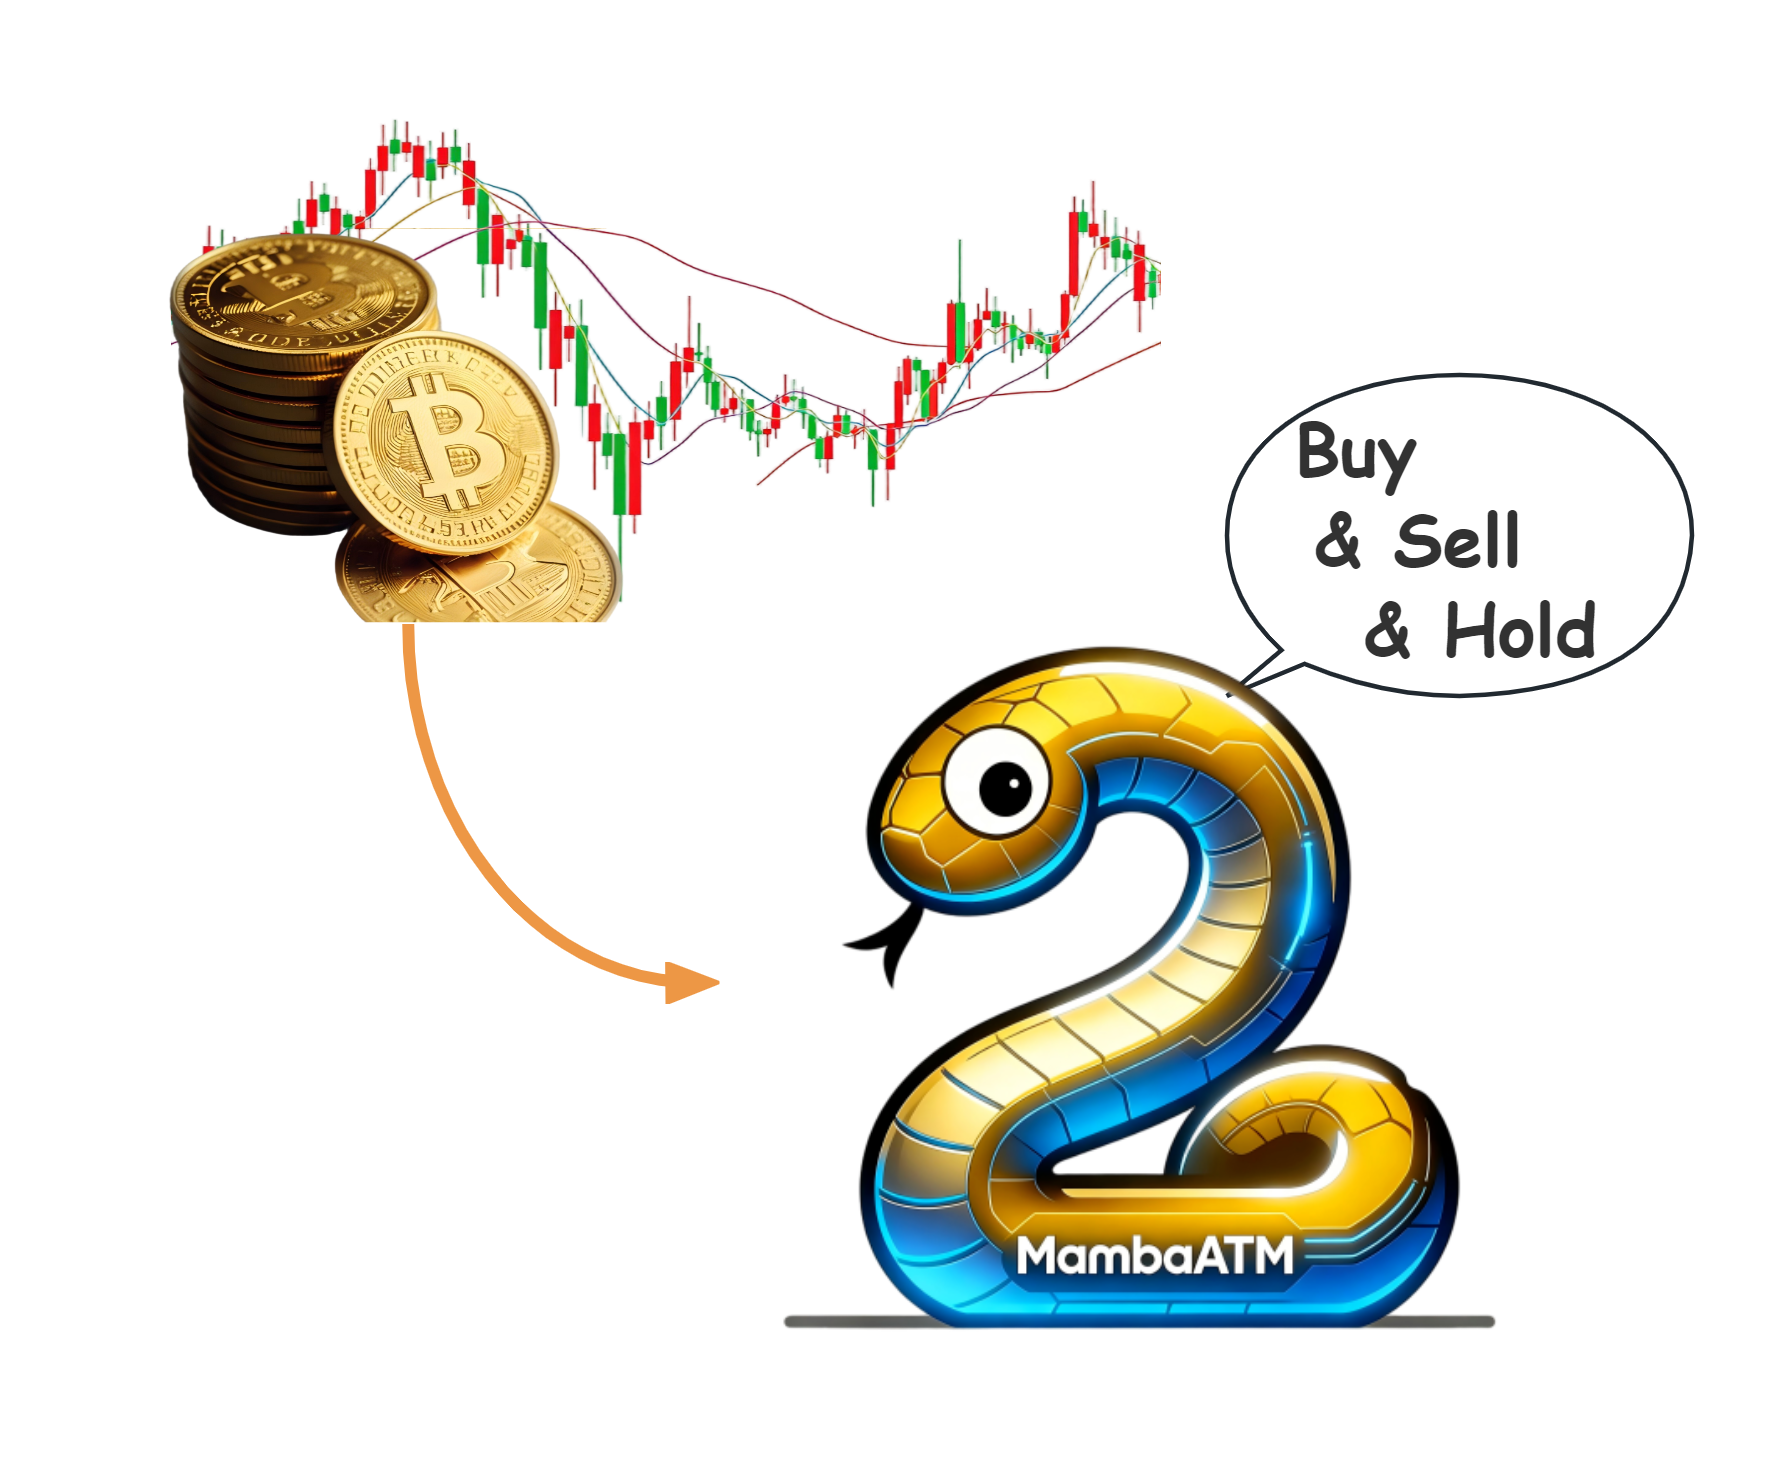
\includegraphics[width=0.72\textwidth]{figs/task}
	\caption{The task setting. A price series for one stock enters MambaATM, which maps a look-back
		window of the recent past to a trading decision. The decision layer is drawn here with the
		three outcomes of the original design, and the evaluation of Section~\ref{sec5} reduces it
		to one binary direction per stock, from which the long-flat rule and the equal-weight
		portfolio follow.}\label{fig:task}
\end{figure}

The mainstream architectures each address part of the modelling problem. Recurrent networks with
gating alleviate the vanishing-gradient difficulty of long-range dependence but process a sequence
serially~\citep{LSTM}, multilayer perceptrons fit nonlinear features cheaply but model time only
implicitly~\citep{MLP}, and attention selects relevant history adaptively but pays a quadratic cost
in the sequence length~\citep{vaswani2017attention}. Structured state-space models~\citep{gu2020hippo,
	gu2022efficiently} and their selective successors~\citep{gu2024linear,Mamba2} scale close to linearly
and carry a recurrent state, at the price of a less explicit selection mechanism. Combining the two
is therefore a natural design, and a number of recent works do so~\citep{kadiyala2025mamba,
	zhao2026cryptomamba}. In practice the combination is easier to build than to justify, because the
evidence that favours it is usually collected without pricing the positions that it implies, and this
paper takes the combination as a case and asks what survives a protocol that a referee can check.

However, three questions about this class of result are not settled by the literature. First, whether
a reported advantage of a hybrid architecture survives when the trivial references are in the table,
because on a daily equity panel a majority-class rule and buy and hold are genuine competitors.
Second, whether the mechanism that an architecture is credited with is the mechanism that its code
implements, because a hybrid model can be described by the paper and built differently by the
repository. Third, whether the target and the holding period that these comparisons normally use are
the ones that carry the signal, because the absolute daily direction of a single stock is only one way
to pose the problem, and changing the target can move the same model from losing to profitable
without any change to the model itself.

Although both families of models are by now well developed, and although the cross-sectional
literature has long known that the choice of target decides what a model is measuring, the three
questions fall between them. The systematic-comparison literature reports accuracy and error metrics
on prices~\citep{hu2025fintsb,MAEandR2,RMSE}, the choice of metric is itself
studied~\citep{f1-score,recall}, the state-space literature reports long-range benchmarks on
non-financial sequences, and the hybrid works report a gain over their own baselines without pricing
the positions that the gain implies. We address all three questions on one panel of A-share equities.
First, we specify the architecture exactly as it is implemented and report where that specification
differs from earlier descriptions of it, so that the mechanism is a fact about the code rather than a
claim about the design. Second, we audit the protocol instead of asserting it, with a causality
regression test, a check on where modules are constructed, a leakage check on the standardiser and
integrity checks on the panel itself. Third, we evaluate ten models per stock under walk-forward
folds with a purge, and we report every result against the majority class and against buy and hold at
four cost levels. Fourth, we decompose the next-day return into its overnight and intraday legs and
change the target from the absolute direction of one stock to the cross-sectional rank, holding the
models fixed, which locates where the signal is and what it is worth once the positions are priced.

The paper's contributions are as follows.

\begin{enumerate}
	\item \textbf{An architecture specified as it is implemented.} MambaATM runs a causal attention
	branch and a selective state-space branch over the same look-back window and mixes their outputs
	with a learned sigmoid gate, $g \odot h_{\text{ssm}} + (1-g) \odot h_{\text{att}}$. An earlier
	version of this work described the mechanism as \emph{attention guiding the state update} of the
	state-space branch, which is not what the code did, so we implement both and report the
	comparison, and it is not flattering to the stronger claim (Section~\ref{sec:ablation}).
	
	\item \textbf{A protocol that is audited rather than asserted.} The evaluation rests on a
	reconstructed panel of \nStocks{} A-share stocks covering \firstDate{} to \lastDate{}
	(\nStockDays{} usable stock-days), retrieved from a public source and screened for impossible
	adjusted moves, and four checks are run and reported on it, namely a causality regression test, a
	check that no module is constructed inside a forward pass, a leakage check on the standardiser
	and a set of integrity checks on the panel itself. Each of them caught a defect in the earlier
	version of this work (Section~\ref{sec:audits}).
	
	\item \textbf{An evaluation that includes the baselines the claim needs, and the references it has
	to beat.} Ten models are compared, which are eight baselines and the two variants of the
	proposed model, the baselines being MLP, LSTM, causal attention with a causal convolution,
	DLinear~\citep{zeng2023dlinear}, PatchTST~\citep{nie2023patchtst},
	iTransformer~\citep{liu2024itransformer}, TimesNet~\citep{wu2023timesnet} and the selective
	state-space branch on its own. Each is evaluated per stock with five expanding-window
	walk-forward folds and a one-day purge, the results are reported against the majority class and
	buy and hold with Friedman and Holm-corrected Wilcoxon
	tests~\citep{friedman1937use,wilcoxon1945individual}, and costs are charged per position change at
	four levels, because the sign of the net return of a daily strategy depends on them.
	
	\item \textbf{Where the signal is, and what it is worth.} The next-day return is decomposed into
	an overnight leg and an intraday leg, and the target is changed from the absolute direction of
	one stock to the cross-sectional rank of the same panel. The overnight leg carries
	\dilutionRatio{} times the close-to-close information coefficient, which is what the
	close-to-close target was diluting, but a twenty-nine-factor library explains \rSquaredLo{} to
	\rSquaredHi{} of the cross-sectional variance of the models, and pricing the positions with
	commission, time-varying stamp duty, square-root impact and borrow leaves weekly rebalancing on
	the liquid half as the only viable configuration (Section~\ref{sec5}).
\end{enumerate}

The result is reported as measured. On this panel the eight baselines span \rangeAcc{} percentage
points of accuracy, from \accWorst{} to \accBest, against a majority-class rate of \accMaj, and not
one of them reaches that rate. MambaATM is fifth of ten on mean rank at \accProp{}
($\pm$ \accPropSd), the most accurate model is \accBestName{} at \accBest, and the models closest
behind it are \accLSTM{} and \accAtt{}. At the portfolio level buy and hold loses \portAnnBH{} a year
over these test blocks, only \nPortProfit{} of the ten models earn a positive return at the base
cost, and MambaATM is not one of them, since it returns \portAnnProp{} a year at a Sharpe of
\portShProp. The guided variant does not improve on the gate. Changing the target changes the answer
rather than the model. On the cross-sectional rank the same models reach an information coefficient
of \icCcProp{} on the close-to-close return and \icOnProp{} on the overnight leg, and a weekly
long-short book on the liquid half returns \netWk{} a year net of costs, but the factor library
accounts for most of it, the best configuration is three quarters cheap factors, and daily
rebalancing is destroyed by impact. The two halves of that answer, the negative one and the
conditional one, are what Sections~\ref{sec5} and~\ref{sec:discussion} set out.

The remainder of the paper is organised as follows. Section~\ref{sec2} reviews automated trading
models, state-space sequence models, cross-sectional prediction and the cost literature.
Section~\ref{sec3} fixes notation, states the assumptions that are used, restates the complexity of
the two branches, and describes the audits. Section~\ref{sec:method} specifies the architecture as
implemented, including the guided variant, and defines the three labels that the two targets use.
Section~\ref{sec5} reports the experiments, first on the absolute direction of a single stock and then
on the cross-sectional rank, the factor library and the cost of trading either. Section~\ref{sec6}
concludes with the limitations that the results impose.

\section{Related Work}\label{sec2}

\subsection{Automated trading and cross-sectional prediction}

Automated trading models aim to model financial time series accurately enough to generate stable
signals, and to convert those signals into positions under risk control ~\citep{chen2025analysis,
	sarmento2019enhancing}. The literature has moved from rule-based systems to deep learning in three
stages.

Early work mined technical rules with genetic algorithms ~\citep{allen1999using} or combined
fundamental and technical features with support vector machines and fixed stop-loss rules
~\citep{mani2016stock,SVM}. Such systems work while the market structure is stable and fail when it
is not, because the feature space is designed by hand and the decision rule does not adapt
~\citep{li2025rd}.

Deep learning replaced the rule with a learned mapping. LSTM became the default for price-trend
prediction ~\citep{ahmed2026explainable,akgun2024stock}; MLPs remain competitive on tabular
factor problems and are cheap ~\citep{MLP,zhao2026cryptomamba}; attention models integrate
multi-source information well but pay a quadratic cost in sequence length
~\citep{vaswani2017attention,kadiyala2025mamba}. Chen et al. compared loss functions, quasi-Newton
optimisation, fully connected networks and support vector machines for frequent trading and found
the network variants more accurate and more robust ~\citep{chen2025analysis}; Sarmento and Horta
combined clustering with ARMA and LSTM to reduce drawdown by 75\% in a falling market, without
modelling transaction costs ~\citep{sarmento2019enhancing}.

More recent work adds agents, data-centric pipelines and interpretability. The R\&D-Agent-Quant
framework automates factor mining and strategy generation ~\citep{li2025rd}, the FinTSB benchmark
provides a unified evaluation process across market states ~\citep{hu2025fintsb}, and
LSTM-Attention-SHAP couples prediction with feature-level explanation ~\citep{ahmed2026explainable}.

Two gaps motivate this paper. First, reported gains are rarely tested against the trivial
references, so a model that predicts the majority class on a rising market looks accurate. Second,
costs and position changes are often either absent or modelled at a single rate, while the sign of
the net return of a daily strategy is decided by them ~\citep{frazzini2018trading}.

The modern empirical literature predicts the cross-section of returns rather than the direction of one
stock, because the market factor is differenced out and the target becomes relative performance. The
canonical demonstration that machine learning improves on linear factor models is
~\citet{gu2020empirical}, whose out-of-sample $R^2$ values for monthly stock returns are a few tenths
of one per cent, which is large in that literature. Our panel is daily, the horizon is one day, and
our metric is a rank information coefficient, but the same logic applies, since a small positive rank
correlation is an economically meaningful finding, and the interesting question is not whether it
exists but whether it is new.

That question is answered against a factor library, and the answer depends on how large the library
is. Our library has twenty-nine members computed from the eight columns the panel carries. They are
reversals at one, five and twenty days, momentum, several volatility measures, the shape of the
daily bar, liquidity and turnover measures, the overnight and intraday decomposition of the stock's
own returns, and market exposure. Every member is oriented so that the literature's prior has the
higher score on the higher return. Where a member is a linear combination of the others its residual
is computed with that member left out of its own regression, so the comparison is not decided by
construction.

\subsection{State-space models, the return decomposition and the cost of trading}

State-space models describe a sequence through a latent state whose evolution is linear and whose
parameters are usually fixed. HiPPO turned memory into online function approximation with
orthogonal polynomial bases ~\citep{gu2020hippo}, and S4 made the recurrence computable by
diagonalising the state transition and adding a low-rank correction, reducing the cost from
quadratic to $\mathcal{O}(N+L)$ ~\citep{gu2022efficiently}. The transition matrix is fixed, however,
and cannot react to the content of the input ~\citep{popov2026scaling}.

Mamba makes the parameters input-dependent, which restores content-aware selection while keeping a
linear cost and a hardware-aware parallel scan ~\citep{gu2024linear}. Mamba2 shows that the same
computation can be written as a structured matrix multiplication with a semiseparable mask, which
allows a chunked implementation ~\citep{Mamba2}. In finance, state-space models have been used for
volatility prediction on cryptocurrencies, with reported reductions in absolute error of 23.7\%
~\citep{zhao2026cryptomamba}, and for high-frequency throughput, with reported latency in the
hundreds of microseconds ~\citep{popov2026scaling}. Lightweight adaptation and multimodal fusion have
also been explored ~\citep{annepaka2025large,kadiyala2025mamba}.

The design question this paper addresses is what the attention branch should do to the state-space
branch. The submitted version of this work claimed that attention modulated the state update; the
implemented model mixed the branch outputs with a gate. Both are defensible designs, they are not
the same design, and the difference is measurable. Section~\ref{sec:method} implements both and
Section~\ref{sec:ablation} reports which one the panel prefers.


That the two legs of a daily return behave differently is established. ~\citet{berkman2012paying}
document that overnight returns are driven by retail attention and that buying at the open is
expensive; ~\citet{lou2019tug} formalise the tension between the two legs and show that they carry
different expected returns, with different clienteles trading each. Our result is a different use of
the same decomposition, in that we relocate where predictive information sits in a machine-learning
evaluation, and we show that the close-to-close metric is a diluted version of the overnight one
rather than an independent quantity.

The practical reading of the decomposition, that entering at the open forfeits the predicted jump,
is exactly the cost ~\citet{berkman2012paying} describe, and our contribution is to quantify it in
a cost model that also carries impact and borrow, and to show that a weekly book traded at the close is
the configuration that survives.


Costs decide the sign of a daily strategy, and the literature on trading costs and on the capacity of
anomalies is the relevant benchmark ~\citep{frazzini2018trading}. We model the components the Chinese
market actually charges, which are commission on both sides, the stamp duty on the sell side at the
rate in force at the time, a square-root impact term that grows with the size of the book relative to
the name's turnover value, and a borrow fee on the short leg. Reporting the break-even commission and
the break-even book size, rather than one net return at one assumed fee, follows the same instinct as
the work on backtest overfitting and non-normal performance measures ~\citep{bailey2014deflated},
where an assumed rate is replaceable by its critical value.

\section{Preliminary}\label{sec3}

This section fixes notation, states the assumptions actually used, restates the complexity of the
two branches without over-claiming, and defines the audits that the protocol has to pass.

Let the look-back window be $X \in \mathbb{R}^{B \times T \times D}$, with batch size $B$, window
length $T$ and feature dimension $D$; the model emits one logit per window. The attention branch
uses $Q,K,V \in \mathbb{R}^{B \times T \times d_k}$ with head dimension $d_k$ and $H$ heads. The
state-space branch has state dimension $N$, heads $h$, discretisation step $\Delta$, input matrix
$B_t$, output matrix $C_t$, learned transition $A$ and skip connection $D$. The gate is
$g \in (0,1)^{d}$. Costs are quoted per position change, so a round trip from flat to long and back
costs twice the quoted rate.

\subsection{Assumptions}

We state only what the experiments rely on, and we state it in measurable terms.

\begin{Assumption}[Local stationarity of the look-back window]\label{A1}
	Over a window of $T=\seqLen$ trading days the series is locally stationary, so its mean and
	variance are approximately constant and the autocovariance depends on the lag. The assumption is
	weak enough to be testable, and Section~\ref{sec:audits} reports the measured autocorrelation of
	daily returns on the panel, which averages \acfMean{} at lag one over the \nStocks{} stocks and
	ranges from \acfMin{} to \acfMax{}. A small positive lag-one autocorrelation in individual stocks
	is a documented property of thinly traded and partially adjusting markets rather than a defect,
	and we report the measured value instead of asserting that returns are uncorrelated.
\end{Assumption}

\begin{Assumption}[Causality of the model]\label{A4}
	The output of the model for a window ending at day $t$ depends only on data up to day $t$. Inside
	the window, the attention weights are masked to be lower triangular and the depthwise convolution
	is left-padded, so position $\tau$ never reads beyond $\tau$. This is verified by regression test
	rather than asserted (Section~\ref{sec:audits}).
\end{Assumption}

\begin{Assumption}[Trading environment]\label{A5}
	Positions are long or flat, without leverage; one position is held per stock; the portfolio is
	equal-weighted across the stocks that have a signal on a given day. A change of position is
	charged $c$ one way, covering commission, stamp duty on the sell side and slippage. Results are
	reported for $c \in \{0, 10^{-3}, 1.5\times10^{-3}\}$ and for zero cost, so the reader can see how
	much of any result depends on the assumption.
\end{Assumption}

\begin{Assumption}[Feature information]\label{A2}
	Every feature carries some information about the next-day return. On the panel the largest
	absolute rank correlation between any single feature and the next-day return is \maxRankCorr{}
	over all stocks and features, with a median of \medRankCorr{}, so the assumption holds but only
	weakly, and it is reported as measured rather than used as a guarantee. It exists here to make
	explicit that the task is not one where a feature almost determines the label; if it did, the
	comparison of architectures would be uninformative.
\end{Assumption}

Assumption~A3 of the earlier version of this work fixed the initialisation distribution of the
input and output matrices of the state-space branch. It is not used anywhere in the analysis, and it
is dropped; the initialisation that the code actually uses is stated in Section~\ref{sec:method}.

\subsection{Complexity of the two branches}

\begin{Lemma}[Causal self-attention]\label{L1}
	Multi-head causal self-attention over a window of length $T$ costs
	$\mathcal{O}(B T d_k^2 + B T^2 H)$, in which the projections are linear in $T$ and the pairwise
	scores are quadratic. Causal masking does not change the order. This restates the standard result
	~\citep{vaswani2017attention} and is not re-derived.
\end{Lemma}

\begin{Lemma}[Selective state-space branch]\label{L2}
	The selective scan over the window costs $\mathcal{O}(B T D N)$ in operations, and the chunked
	implementation used here adds no asymptotic factor, because the sequence is split into blocks whose
	length divides $T$ and the intra-block term, the inter-block state term and the state decay are
	each computed with matrix products over blocks. The earlier version of this work quoted
	$\mathcal{O}(B T D N \log T)$; the logarithmic factor belongs to the parallel scan of the original
	formulation, not to the chunked decomposition used in the implementation, and we do not claim it.
\end{Lemma}

\begin{Lemma}[Whole model]\label{L3}
	The model of Section~\ref{sec:method} computes both branches over the same window. Its cost is
	$\mathcal{O}(B T^2 H + B T d_k^2 + B T D N)$, in which the quadratic term is quadratic in the
	\emph{window length} $T$, not in the length of the series.
\end{Lemma}

\begin{proof}
	Both branches read $X$ and each contributes its own term, from \Cref{L1} and \Cref{L2}. Nothing in
	the gate is superlinear in $T$, since it is a linear map of the two branch outputs followed by a
	sigmoid.
\end{proof}

The distinction matters for the claim that the earlier version made. That version stated that the
quadratic term of attention is \emph{eliminated}, because attention was said to be used only to
generate the state parameters. The implemented model keeps a real attention branch, so the term is
present and bounded by the window length, which is fixed at \seqLen{} in all experiments. On a
long series the state-space branch is the one whose cost grows with the series; on a fixed window
both branches are cheap, and the measured wall-clock times in Section~\ref{sec:efficiency} show the
difference between the models to be a factor of a few rather than an order of magnitude.

\subsection{Audits}\label{sec:audits}

Four checks are run before any result is used, and each is reported with its outcome. Their purpose
is to make the protocol falsifiable rather than to decorate it.

\textbf{A1. Causality.} Take a window, randomise the parameters of the sequence model, and perturb
the inputs at all positions from a cutoff onwards. The outputs at positions before the cutoff must
be unchanged. For the branch used here the maximum change is exactly zero for the attention branch
with a causal convolution, for the selective state-space branch, and for both fused variants. The
test has teeth, because it fails with a change of $4\times10^{-3}$ to $7\times10^{-3}$ for the
architecture of the earlier version, which used symmetric padding in a depthwise convolution and
therefore let position $t$ read $t+1$.

\textbf{A2. No module built inside a forward pass.} A layer constructed inside \texttt{forward} is
not in the parameter list of the optimizer, so its weights are re-randomised on every call,
including at evaluation time. The check builds each model, records the identities of its parameters,
runs a forward pass and requires the set to be unchanged. It is unchanged for every model reported
here; it was not for the earlier version, whose residual projection was created inside
\texttt{forward}.

\textbf{A3. Standardisation without leakage.} The standardiser is fitted on the training block of
each fold. The check rewrites the test block and requires the standardised training block to be
identical, then rewrites the training block and requires the standardised test block to change. The
earlier version z-scored every column over the whole sample, so test-period statistics entered the
training inputs; the check fails on that pipeline and passes on this one.

\textbf{A4. Panel integrity.} For every stock the return column must agree with the return implied
by the price columns, the previous-close column must equal the previous row's close, no feature may
be constant, and no adjusted daily move may exceed the exchange limit band used for screening. On
the panel used here the correlation between the quoted return and the price-implied return is
$1.000$ for all \nStocks{} stocks with a mean absolute difference of $5\times10^{-17}$, the
previous-close identity holds for every row, no feature column is constant, and the largest adjusted
daily move is 11.5\%. On the dataset of the earlier version, by contrast, the quoted return and the
price-implied return correlated between $-0.15$ and $+0.03$, 248 of 258 columns were identically
zero, and the number of rows was 500 rather than the 2{,}435 described in the text.

\section{Methods}\label{sec:method}

\subsection{Architecture as implemented}

MambaATM takes a window $X \in \mathbb{R}^{B \times T \times D}$ and produces one logit. It has two
branches and a gate.

\textbf{Attention branch.} A linear map takes $X$ to $h \in \mathbb{R}^{B \times T \times d}$ with
$d = 64$. Single-head attention with a lower-triangular mask is applied to $h$,
$\mathrm{softmax}(\mathrm{mask}(QK^\top/\sqrt{d}))V$, and the result is added to a depthwise
convolution of $h$ with kernel 3 that is \emph{left}-padded so that the convolution is causal. The
sum is layer-normalised; its last position, $h_{\text{att}}$, is the branch representation.

\textbf{State-space branch.} The same window enters a selective state-space block. A linear map
produces two halves, of which one is convolved causally and passed through SiLU, and from the result
a low-rank projection produces the discretisation step and the input and output matrices, so
$\Delta_t$, $B_t$ and $C_t$ all depend on the input. The transition is diagonal and learned as
$\mathtt{A\_log} \in \mathbb{R}^{h}$ with $A = -\exp(\mathtt{A\_log})$, together with a learned skip
$D$. The recurrence is computed with the chunked decomposition of the structured state-space duality
~\citep{Mamba2}, using the reference minimal implementation of ~\citet{Mamba2} for the intra-block
term; the sequence is padded to a block length that divides $T$. The output is gated by a SiLU of
the second half and projected back to $d$ dimensions; its last position is $h_{\text{ssm}}$.

\textbf{Gate.} The two representations are concatenated and mapped by a linear layer with a sigmoid,
$g = \sigma(W[h_{\text{att}}; h_{\text{ssm}}] + b) \in (0,1)^d$, and the fused representation is
\begin{equation}\label{eq:gate}
	h = g \odot h_{\text{ssm}} + (1-g) \odot h_{\text{att}},
\end{equation}
from which a linear head produces the logit. Equation~\eqref{eq:gate} is a convex combination per
channel, so the gate chooses how much of each branch to keep, and it does \emph{not} modify the state
update of the state-space branch. This is the mechanism the earlier version of this work described
as ``attention guides the state update'', and the description was of a different model.
Fig.~\ref{fig:framework} draws the architecture as it was described. Table~\ref{tab:claim} lists the
differences between that description and the implementation, because the review identified them and
because the same table is the reason the guided variant is reported separately.

\begin{figure}[tbp]
	\centering
	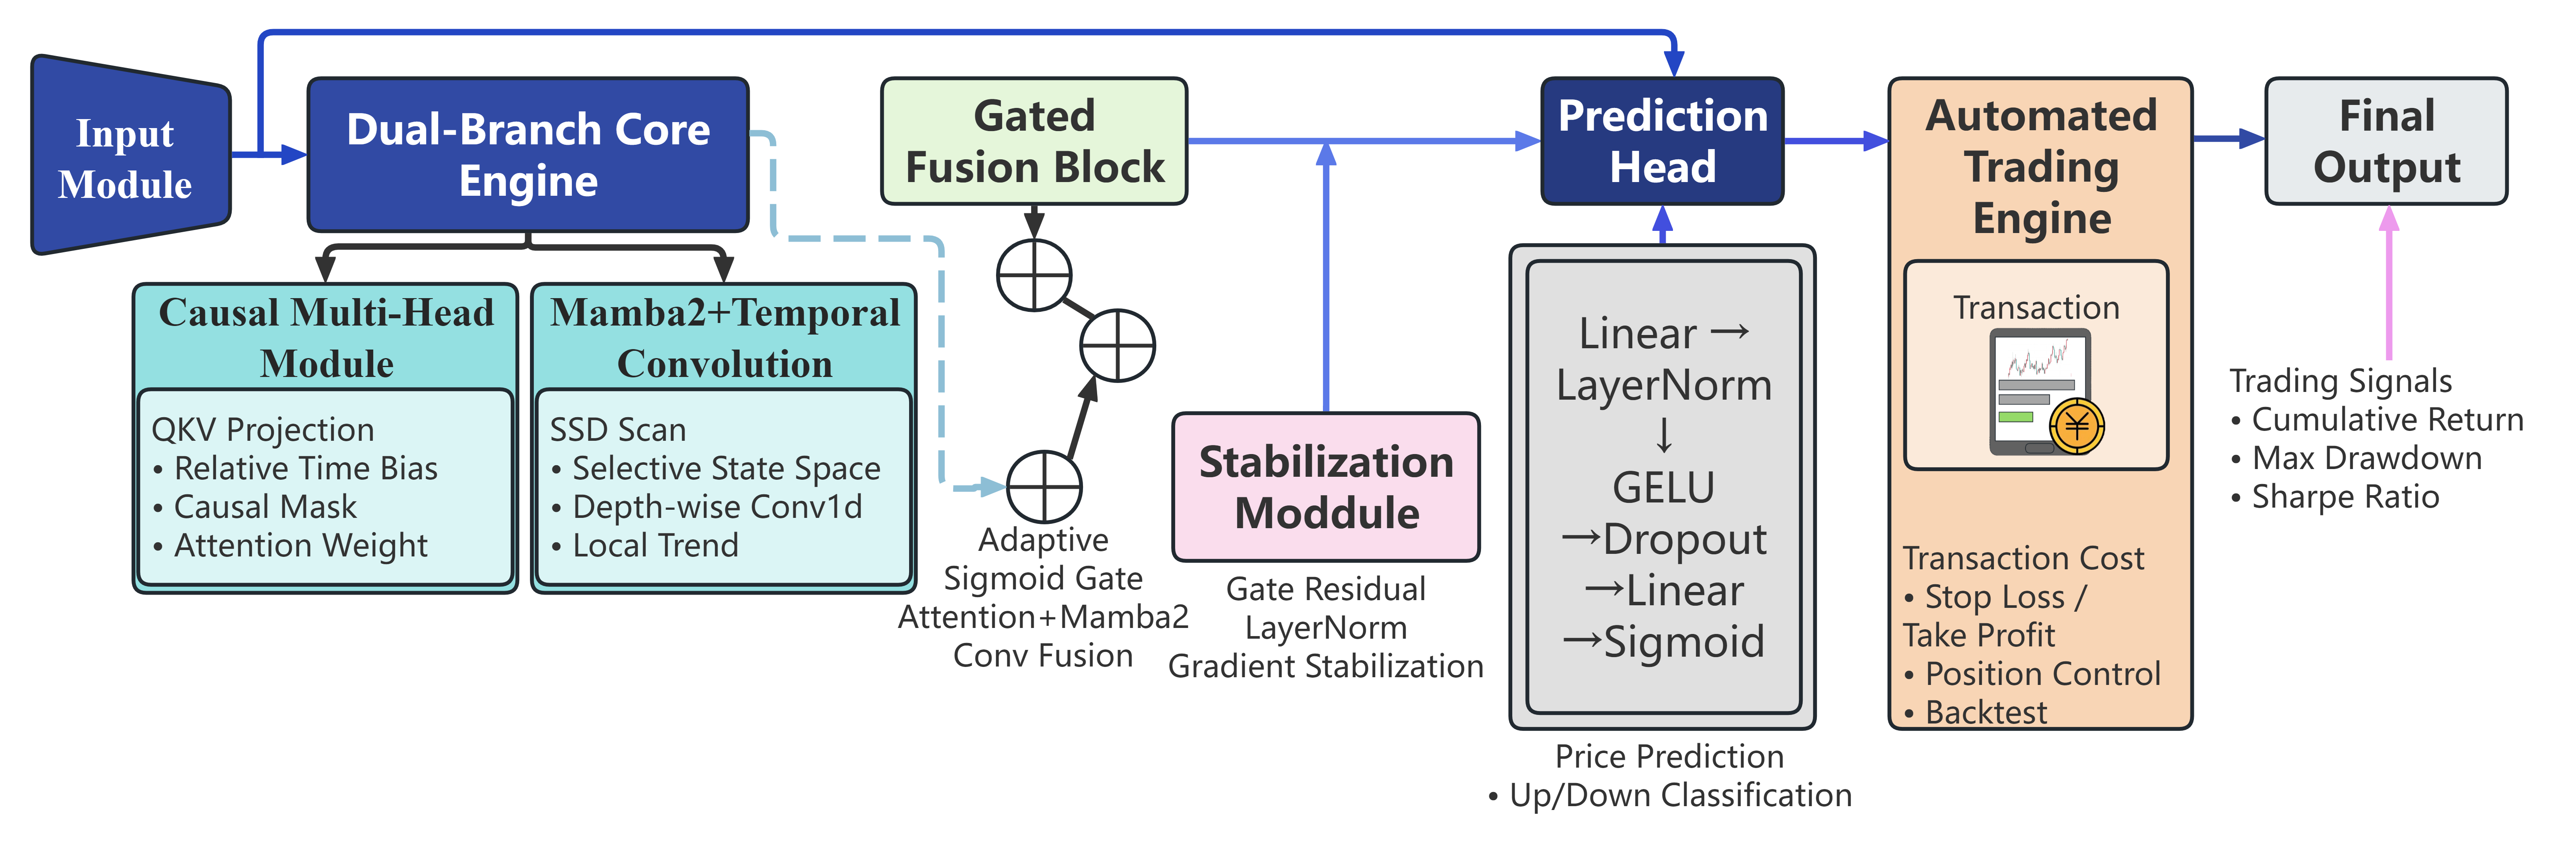
\includegraphics[width=\textwidth]{figs/framework}
	\caption{The architecture as described. A window of input features enters a dual-branch core
		that holds a causal multi-head attention branch and a selective state-space branch. The two
		representations are combined by a gated fusion block, then stabilised, mapped to an output
		and passed to the trading layer. Section~\ref{sec:method} specifies the configuration that
		was evaluated, and the rows on which that configuration differs from this description are
		listed in Table~\ref{tab:claim}. The price-regression output and the stop-loss and
		take-profit rules drawn in the trading layer are not part of the evaluation reported here,
		which uses the long-flat rule and the equal-weight portfolio of Section~\ref{sec5}.}
		\label{fig:framework}
\end{figure}

\begin{table}[tbp]
	\centering
	\caption{The architecture as described in the earlier version of this work, and as implemented in the version evaluated here. Each row is checked by a script in the code release; the rows that differ are the reason the guided variant is reported as a separate experiment.}
	\label{tab:claim}
	% The architecture as it was described in the earlier version of this work, and as it is implemented
% here. Every entry in the right-hand column is reproduced by a script in the code release.
\small
\setlength{\tabcolsep}{4pt}
\begin{tabularx}{\textwidth}{@{}>{\raggedright\arraybackslash}p{0.22\textwidth}
	>{\raggedright\arraybackslash}X>{\raggedright\arraybackslash}X@{}}
	\toprule
	\textbf{Aspect} & \textbf{Earlier description} & \textbf{Implementation evaluated here} \\
	\midrule
	Fusion & Attention guides the state update of the state-space branch; the two branches are not
	concatenated. &
	The two branch outputs are mixed by a learned sigmoid gate,
	$g \odot h_{\text{ssm}} + (1-g)\odot h_{\text{att}}$. The gate weights the outputs; it does not
	touch the state update. \\
	\addlinespace
	Guidance & Stated as the defining mechanism of the proposed model. &
	Implemented as a separate variant, with zero-initialised projections that scale the
	discretisation step and shift the input and output matrices. Reported as an ablation. \\
	\addlinespace
	Attention branch & Implied absent in the complexity argument, since only the QKV projection was
	said to be retained. &
	A full causal attention branch is present and contributes its output to the fused representation. \\
	\addlinespace
	Complexity & $\mathcal{O}(B T D N \log T + B T d_k^2)$, with the quadratic term described as
	eliminated. &
	$\mathcal{O}(B T^2 H + B T d_k^2 + B T D N)$: the quadratic term is present and bounded by the
	window length $T$. \\
	\addlinespace
	Causality & ``Every model passes with a change of exactly zero.'' &
	Measured. The causal variants pass with a change of exactly zero; the architecture of the earlier
	version fails, with a change of $4\times10^{-3}$ to $7\times10^{-3}$, because of symmetric
	padding in a depthwise convolution. \\
	\addlinespace
	Weights & Not discussed. &
	No module is constructed inside a forward pass, verified by comparing the parameter set before
	and after a forward pass. The earlier version built a residual projection inside
	\texttt{forward}, which left it untrained. \\
	\addlinespace
	Data & Four unnamed stocks, 2{,}435 rows each, six features, 2015--2025, normalised to $[0,1]$. &
	\nStocks{} named A-share stocks, \nStockDays{} usable stock-days, eight features, \firstDate{} to
	\lastDate{}, standardised inside each fold on the training block only. \\
	\bottomrule
\end{tabularx}

\end{table}

\subsection{The guided variant, and why it is reported separately}

The mechanism the earlier version claimed is a defensible design, so we implement it as well. In the
guided variant the attention representation at each position, $h^{\text{seq}}_{\text{att}} \in
\mathbb{R}^{B \times T \times d}$, is passed to the state-space branch, where three zero-initialised
projections produce
\begin{equation}\label{eq:guided}
	\tilde{\Delta}_t = \Delta_t \odot \bigl(1 + \tanh(W_\Delta h^{\text{seq}}_{\text{att},t})\bigr),
	\qquad
	\tilde{B}_t = B_t + W_B h^{\text{seq}}_{\text{att},t},
	\qquad
	\tilde{C}_t = C_t + W_C h^{\text{seq}}_{\text{att},t}.
\end{equation}
Because the three projections start at zero, the guided variant begins exactly as the plain branch
and differs only in what training chooses to do with the modulation. Guided and unguided therefore
differ in one capacity, not in initialisation or in size by more than
\paramGuided{} against \paramProposed{} parameters. The comparison is reported in
Section~\ref{sec:ablation}, and the outcome is that the modulation does not pay for itself.

\begin{algorithm}[H]
	\caption{MambaATM, as implemented}
	\label{alg:mambaatm}
	\begin{algorithmic}[1]
		\Require window $X \in \mathbb{R}^{B \times T \times D}$, hyperparameters $\Theta$,
		guided flag $\in \{\text{true},\text{false}\}$
		\Ensure logit $\hat{y} \in \mathbb{R}^{B}$
		\State $h \leftarrow \mathrm{Linear}(X)$
		\State $A_{\text{seq}} \leftarrow \mathrm{CausalAttention}(h) + \mathrm{CausalConv1d}(h)$
		\State $h_{\text{att}} \leftarrow \mathrm{LayerNorm}(A_{\text{seq}})[:, -1]$
		\If{guided}
		\State $(\tilde{\Delta}, \tilde{B}, \tilde{C}) \leftarrow
		\mathrm{Modulate}(\Delta, B, C, \mathrm{LayerNorm}(A_{\text{seq}}))$
		\Comment{Eq.~\eqref{eq:guided}}
		\Else
		\State $(\tilde{\Delta}, \tilde{B}, \tilde{C}) \leftarrow (\Delta, B, C)$
		\EndIf
		\State $S \leftarrow \mathrm{ChunkedSelectiveScan}(X, \tilde{\Delta}, \tilde{B}, \tilde{C}, A, D)$
		\State $h_{\text{ssm}} \leftarrow \mathrm{Linear}(S[:, -1])$
		\State $g \leftarrow \sigma(\mathrm{Linear}([h_{\text{att}}; h_{\text{ssm}}]))$
		\State $h \leftarrow g \odot h_{\text{ssm}} + (1-g) \odot h_{\text{att}}$
		\Comment{Eq.~\eqref{eq:gate}}
		\State \Return $\mathrm{Linear}(h)$
	\end{algorithmic}
\end{algorithm}

\subsection{Training protocol}

Each stock is split into five expanding-window folds. The first test block begins after 40\% of the
windows, the folds then partition the remaining windows, and a one-day purge is removed from the end
of each training block, so the last training label cannot be the first test label. Within a fold the
standardiser is fitted on the training block only, the last 10\% of the training windows are held out
in time order for early stopping, and the model is restored to the epoch of lowest validation loss
before the test block is predicted. Windows are not shuffled across the fold boundary, and test
windows lie entirely inside the test segment. All models share the same windows, the same fold
boundaries, the same optimiser (Adam, learning rate $10^{-3}$), the same batch size of 64 and the
same maximum of \nEpochs{} epochs with a patience of five. The label of a window is the sign of the
return of the next trading day, and the return used for the trading metrics is that same next-day
return, so no same-day return enters the input or the label.

\subsection{Label definition and the references that a result has to beat}

A daily direction model on a rising market can look accurate by predicting always up, and a daily
trading rule can look profitable by holding the asset. Both are reported for every model and every
stock, namely the majority-class rate of the test blocks, the always-long rate, and the return and
Sharpe of holding the stock over the same test days. A model is only described as predictive here if it
beats the majority class on the same days, and only described as economically useful if it beats buy
and hold net of costs on the same days.

\subsection{The three labels}

For a window ending on day $t$, the supervision for day $t+1$ can be one of three quantities:

\begin{align}
	r^{cc}_{t+1} &= \frac{\text{close}_{t+1}}{\text{close}_t} - 1, &
	r^{on}_{t+1} &= \frac{\text{open}_{t+1}}{\text{close}_t} - 1, &
	r^{id}_{t+1} &= \frac{\text{close}_{t+1}}{\text{open}_{t+1}} - 1 .
\end{align}

They satisfy $r^{cc} = r^{on} + r^{id}$ up to a cross term that is negligible at daily horizons. The
first is what the models are trained on and what the literature reports. The second is the object of
this paper. The third is reported for completeness, with one caveat. Under the T+1 settlement rule of
the Chinese market, a share bought at the open of $t+1$ cannot be sold at the close of $t+1$, so the
intraday leg is not harvestable as a standalone trade by a long-only account. It is measured because
the decomposition needs it, not because it can be traded as stated.

\section{Experiments}\label{sec5}

\subsection{Panel}

The panel is built from daily quotes for \nStocks{} A-share stocks retrieved through a public data
interface ~\citep{baostock}, covering \firstDate{} to \lastDate{}. Prices are forward adjusted for
splits and distributions, so a return computed from two consecutive rows is the return an investor
would have received. Each file carries eight fields used as features, which are open, close, high,
low, volume, turnover value, turnover rate and previous close, plus the quoted close-to-close return.

Three categories of row are removed before modelling, and they are not disjoint. The first row of each
file has no return and no previous close. The last row of each file has no next-day return, so it
carries no label. Rows with zero volume are suspension days, because the stock could not be traded,
the quoted return is zero by construction, and including them would both add untradable observations
and push the label distribution toward ``down''. The first and the last of these are one row per
stock, so \nNoPrevRows{} and \nNoLabelRows{} rows respectively, and the suspensions number
\nSuspDays{}, or \pctSusp{} of all rows. \nOverlapRows{} rows are both a first row and a suspension
day, and they are removed once, so \nRemovedRows{} rows are removed in total and the panel holds
\nStockDays{} stock-days, between \minRows{} and \maxRows{} rows per stock depending on when the stock
was listed, with a median of \medRows{}.

The integrity checks of Section~\ref{sec:audits} are applied to this panel and pass. Table~\ref{tab:panel}
summarises it. Nothing is normalised at this stage, because standardisation is part of the model
pipeline and is fitted inside each fold, so the panel files are the raw adjusted quotes and can be
regenerated from the source with the scripts named in the data availability statement.

\begin{table}[tbp]
	\centering
	\caption{The panel. Rows are removed inside the pipeline rather than in the panel files, so the released panel is exactly what was retrieved and screened.}
	\label{tab:panel}
	\begin{tabularx}{\textwidth}{@{}>{\raggedright\arraybackslash}p{0.42\textwidth}>{\raggedright\arraybackslash}X@{}}
\toprule
\textbf{Property} & \textbf{Value} \\
\midrule
Stocks & 232 \\
Trading days & 2015-01-06 to 2025-12-31 \\
Rows in the files & 610\,988 \\
Rows removed: no previous close (first row of each file) & 232 \\
Rows removed: zero volume (suspension) & 22\,798 (3.7\%) \\
Rows removed: no next-day label (last row of each file) & 232 \\
Rows removed twice, being both a first row and a suspension day & 25\, so the three lines above remove 23\,237 distinct rows \\
Usable stock-days & 587\,751 \\
Usable rows per stock (min / median / max) & 1124 / 2596 / 2671 \\
Features & 8: open, close, high, low, volume, turnover value, turnover rate, previous close \\
Label & sign of the next trading day's close-to-close return \\
Share of up days (mean over stocks) & 0.480 \\
Largest absolute rank correlation, any feature with the next-day return & 0.100 (median 0.043) \\
Lag-one autocorrelation of returns (mean, min, max) & +0.080, -0.034, +0.228 \\
Audit: causality change before the cutoff & 0.000000 for every causal model \\
Audit: modules built inside a forward pass & none \\
Audit: standardiser fitted on the training block only & passes \\
Audit: return column against the price columns & correlation 1.000, mean absolute difference $5\times10^{-17}$ \\
\bottomrule
\end{tabularx}

\end{table}

\subsection{Models compared}

Ten models are evaluated under identical conditions, which are eight baselines and the two variants
of the proposed model. MLP flattens the window and applies
two hidden layers. LSTM uses two recurrent layers with a linear head on the last state. Attention is
the mask-only variant of the branch in Section~\ref{sec:method}, and Attention+conv adds the causal
depthwise convolution. DLinear ~\citep{zeng2023dlinear} decomposes the window into a moving-average
trend and a remainder and maps each to the output with a single linear layer. PatchTST
~\citep{nie2023patchtst} splits each channel into patches, embeds them, and runs a transformer
encoder over the patch sequence. iTransformer ~\citep{liu2024itransformer} inverts the axes and runs
attention across variates, each variate's whole window being one token. TimesNet
~\citep{wu2023timesnet} selects periods from the amplitude spectrum, folds the series into a
two-dimensional tensor and applies inception blocks. The selective state-space branch on its own,
called SSM-only in the tables, is that branch with a linear head, which isolates how much of the
fused model comes from it. MambaATM is
the gated fusion of Eq.~\eqref{eq:gate}, and MambaATM-guided is the modulated variant of
Eq.~\eqref{eq:guided}. Every baseline is adapted to the same binary target by replacing its output
head with a linear map to one logit; nothing else about the input protocol differs.

The parameter count of each model and its measured wall-clock time per stock are reported in
Section~\ref{sec:efficiency}, so the comparison can be read against the cost of each architecture.

\subsection{Overall performance}

Table~\ref{tab:main} reports, for every model, the cross-sectional mean and standard deviation over
the \nStocks{} stocks of accuracy, precision, recall, F1, the correlation between prediction and
return, the total return of the long-flat rule, its Sharpe ratio and its maximum drawdown, all net
of the base cost of $10^{-3}$ one way. The last two rows give the references, which are the
majority-class rate of the same test blocks and buy and hold on the same days. Fig.~\ref{fig:accuracy}
shows the same accuracy stock by stock, and makes the size of the differences in Table~\ref{tab:main}
explicit, since the spread of one model across the cross-section is of the same order as the spread
between models, so a single rank carries less information than the table layout suggests.

\begin{table}[tbp]
	\centering
	\caption{Classification metrics over the panel. Each cell is the mean and standard deviation across the \nStocks{} stocks. The last two rows are the references measured on the same test days. Precision and recall are quoted for the proposed model in the text rather than in this table, because across the panel that pair is governed by the class imbalance, which is itself a result.}
	\label{tab:main}
	% per-stock mean and standard deviation over the panel; generated by make_tables.py
{\footnotesize
\setlength{\tabcolsep}{2pt}
\begin{tabular}{lccc}
\toprule
\textbf{Model} & \textbf{Accuracy} & \textbf{F1} & \textbf{IC} \\
\midrule
MLP & 0.516 $\pm$ 0.019 & 0.354 $\pm$ 0.139 & 0.012 $\pm$ 0.035 \\
LSTM & 0.519 $\pm$ 0.021 & 0.304 $\pm$ 0.163 & 0.011 $\pm$ 0.040 \\
Attention (causal conv) & 0.518 $\pm$ 0.019 & 0.345 $\pm$ 0.145 & 0.009 $\pm$ 0.032 \\
DLinear & 0.521 $\pm$ 0.022 & 0.272 $\pm$ 0.146 & 0.004 $\pm$ 0.035 \\
PatchTST & 0.514 $\pm$ 0.022 & 0.364 $\pm$ 0.130 & -0.000 $\pm$ 0.027 \\
iTransformer & 0.507 $\pm$ 0.019 & 0.409 $\pm$ 0.131 & -0.002 $\pm$ 0.027 \\
TimesNet & 0.513 $\pm$ 0.019 & 0.373 $\pm$ 0.137 & 0.008 $\pm$ 0.042 \\
Selective SSM only & 0.514 $\pm$ 0.022 & 0.355 $\pm$ 0.160 & 0.005 $\pm$ 0.037 \\
\textbf{MambaATM (gated fusion)} & 0.516 $\pm$ 0.021 & 0.356 $\pm$ 0.148 & 0.009 $\pm$ 0.034 \\
MambaATM (guided fusion) & 0.517 $\pm$ 0.021 & 0.340 $\pm$ 0.153 & 0.008 $\pm$ 0.032 \\
\midrule
\emph{Majority class} & 0.528 & -- & -- \\
\emph{Buy and hold} & 0.473 & -- & 1.000 \\
\bottomrule
\end{tabular}
}

\end{table}

\begin{figure}[H]
	\centering
	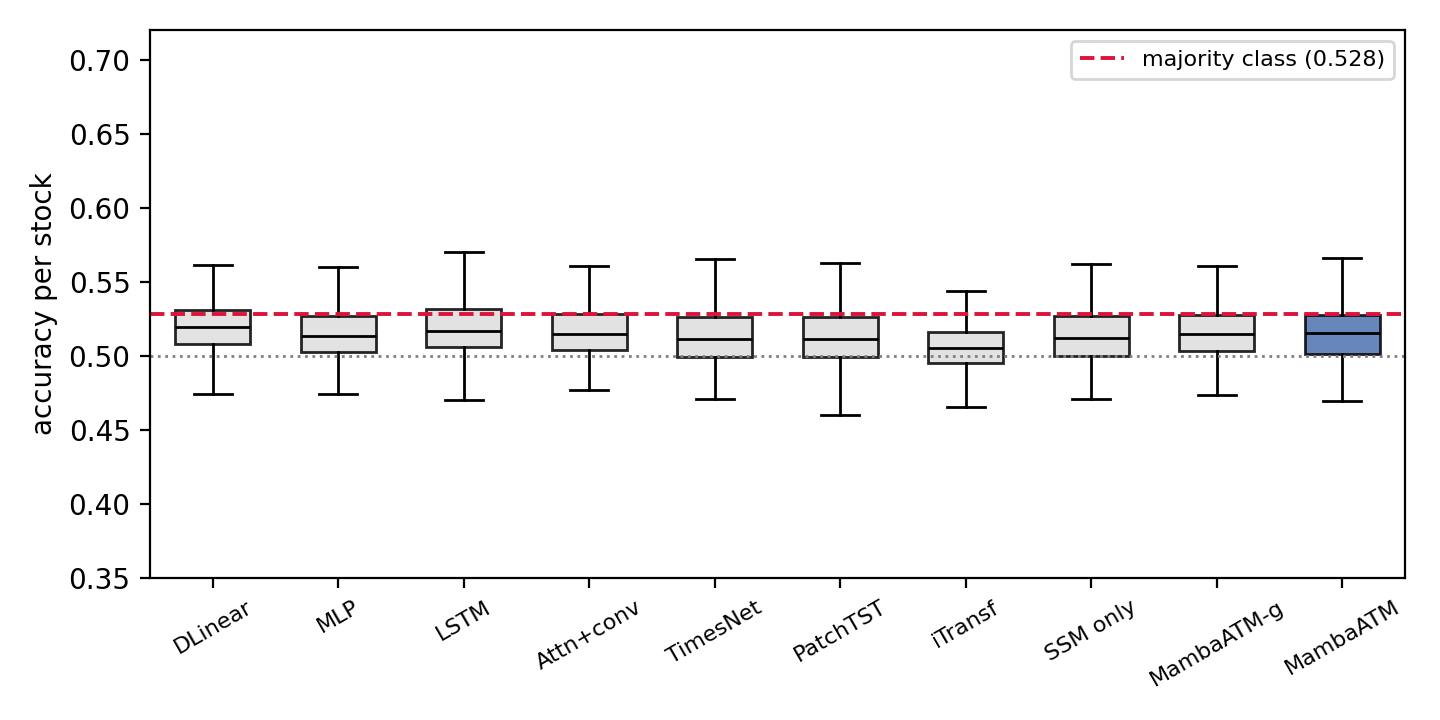
\includegraphics[width=\textwidth]{figs/accuracy_dist}
	\caption{Accuracy of every model on every stock, against the majority-class rate of the same test blocks. The boxes are the cross-section of \nStocks{} stocks; the spread within a model is of the same size as the spread between models, so the ranking in Table~\ref{tab:main} should be read as one band rather than an order.}\label{fig:accuracy}
\end{figure}

Table~\ref{tab:folds} reports the same accuracy fold by fold, which is the rolling-window view the
review asked for. The folds are consecutive in time, so a model whose advantage comes from one
period shows up as a single high column rather than as a consistent one.

\begin{table}[tbp]
	\centering
	\caption{Accuracy of each model in each walk-forward fold, averaged over the panel. The folds are consecutive in time, so a model whose advantage comes from one period shows up as a single high column.}
	\label{tab:folds}
	% mean accuracy per walk-forward fold over the panel
{\scriptsize
\setlength{\tabcolsep}{2pt}
\begin{tabular}{lccccc}
\toprule
\textbf{Model} & \textbf{fold 1} & \textbf{fold 2} & \textbf{fold 3} & \textbf{fold 4} & \textbf{fold 5} \\
\midrule
MLP & 0.511 & 0.514 & 0.521 & 0.523 & 0.510 \\
LSTM & 0.514 & 0.519 & 0.522 & 0.530 & 0.511 \\
Attention (causal conv) & 0.512 & 0.511 & 0.527 & 0.527 & 0.512 \\
DLinear & 0.517 & 0.514 & 0.527 & 0.539 & 0.509 \\
PatchTST & 0.510 & 0.514 & 0.512 & 0.521 & 0.511 \\
iTransformer & 0.506 & 0.510 & 0.512 & 0.500 & 0.509 \\
TimesNet & 0.508 & 0.520 & 0.516 & 0.515 & 0.507 \\
Selective SSM only & 0.519 & 0.506 & 0.519 & 0.519 & 0.509 \\
MambaATM (gated fusion) & 0.512 & 0.516 & 0.519 & 0.519 & 0.514 \\
MambaATM (guided fusion) & 0.512 & 0.515 & 0.522 & 0.521 & 0.514 \\
\midrule
\emph{Buy and hold (return, \%)} & +21.8 & +11.4 & +5.7 & -11.5 & +55.0 \\
\bottomrule
\end{tabular}
}

\end{table}

Three features of the table matter more than the ranking.

\textbf{No learned model reaches the majority class.} The majority-class rate of the test blocks is
\accMaj. The best of the eight baselines, \accBestName, reaches \accBest, and the full set spans
\rangeAcc{} percentage points, from \accWorst{} to \accBest. MambaATM reaches \accProp{} with a
standard deviation across stocks of \accPropSd, which is larger than the gap between the best and the
worst model; its mean rank across the panel is \rankPropAcc{} of ten, so it is distinguishable from
the weakest baseline and from the strongest, and not from the rest. On the sample of stocks where a
model beats the majority class, the best rate in the panel is \beatMajBest{}, held by
\beatMajBestName.

\textbf{Every model collapses toward one class.} The turnover of the MambaATM signal is
\turnProp{} position changes per day, and its recall is \recallProp{} against a precision of
\precProp, so the fused model predicts an upward move most days and is corrected only by the drift of
the sample. The same holds for the other architectures in the table; the highest F1 in the panel is
\fOneBest{} (\fOneBestName), and its accuracy is below the majority-class rate. On this target the
models are not separating signal from noise, and the honest reading of Table~\ref{tab:main} is a
table of models whose accuracy is determined by how well their constant tendency matches the tide of
the test period.

\textbf{Buy and hold is the reference that the economics are measured against.} Holding the average
stock over the same test days earns \retBH{} per stock on average, at a Sharpe of \shBH{} and a
maximum drawdown of \ddBH{}; the per-stock return distribution is wide, with a median of
\medRetBH{}. MambaATM beats buy and hold on \beatBHProp{} of stocks and the majority class on
\beatMajProp{}, and the best model on the majority-class count is not MambaATM. A model earns the
description ``predictive''
here only if it beats the majority class on the same days, and on these data almost none does.

\subsection{Economic evaluation}

Classification accuracy is a poor proxy for the value of a trading rule, because a signal that
changes every day pays the spread every day. Two levels are reported.

At the level of a single stock, the long-flat rule applied to one name returns
\retProp{} on average over the test blocks at a Sharpe of \shProp{} and a maximum drawdown of
\ddProp, with an average turnover of \turnProp{} position changes per day. The dispersion across the
panel is larger than the mean, since the per-stock return has a standard deviation of \retPropSd{}
against a mean of \retProp, so an average return alone would not describe the strategy.

The cost assumption decides the sign of every result at this turnover, which is why the portfolio is
reported at four levels. At the portfolio level, the equal-weight portfolio formed from the positions of a model across the
stocks that have a signal on a given day is the level at which a risk-adjusted claim can be made,
because the idiosyncratic volatility of one name dominates its own Sharpe ratio. Table~\ref{tab:portfolio}
reports annualised return, Sharpe and maximum drawdown of the equal-weight portfolio for each model
at three non-zero cost levels, against buy and hold on the same days, which returns \portAnnBH{} per
year at a Sharpe of \portShBH{} and a maximum drawdown of \portDDBH. On this panel buy and hold loses
money, because the test blocks cover the 2018 and 2022 declines as well as the recoveries, so the
interesting question is not who is profitable but who loses less than holding.

Of the ten models, \nPortProfit{} earn a positive return at this cost, and they are \portProfitNames.
The best of them, \portBestName, returns \portAnnBest{} a year at a Sharpe of \portShBest, and the
other four are barely above zero. MambaATM does not, since it returns
\portAnnPropZero{} a year before costs, \portAnnProp{} at $10^{-3}$ one way and \portAnnPropHigh{} at
$1.5\times10^{-3}$, with a Sharpe of \portShProp, and its signal is the most persistent in the table,
with a per-stock turnover of \turnProp{} changes per day. The signal is almost always long, so the
portfolio inherits the drawdown of the index, \portDDProp, which is the drawdown of buy and hold
itself. The economic conclusion
matches the statistical one. A model whose accuracy sits below the majority-class rate and whose
signal is nearly constant cannot be turned into a strategy by a cost assumption, and
Section~\ref{sec:discussion} draws the conclusion that follows for the architecture.

\begin{table}[tbp]
	\centering
	\caption{Equal-weight portfolio of the panel, net of one-way cost per position change, against buy and hold of the same stocks over the same days.}
	\label{tab:portfolio}
	% equal-weight portfolio of the panel at the base cost of 10 bp one way; the cost
% sensitivity is in Figure 4 and in the numbers quoted in Section 5.4
{\footnotesize
\setlength{\tabcolsep}{3pt}
\begin{tabular}{lcccc}
\toprule
\textbf{Model} & \textbf{ann. \%} & \textbf{Sharpe} & \textbf{max DD \%} & \textbf{turnover} \\
\midrule
Attention (causal conv) & -1.2 & +0.08 & 65.1 & 0.0024 \\
DLinear & +2.9 & +0.24 & 44.4 & 0.0288 \\
MambaATM (gated fusion) & -1.0 & +0.09 & 64.5 & 0.0014 \\
MambaATM (guided fusion) & -1.0 & +0.08 & 63.7 & 0.0033 \\
iTransformer & -0.3 & +0.11 & 62.3 & 0.0014 \\
LSTM & +0.0 & +0.13 & 61.3 & 0.0014 \\
MLP & -0.8 & +0.09 & 61.7 & 0.0033 \\
PatchTST & +2.6 & +0.23 & 54.8 & 0.0052 \\
Selective SSM only & +0.0 & +0.12 & 63.9 & 0.0118 \\
TimesNet & +2.1 & +0.21 & 57.1 & 0.0128 \\
\emph{Buy and hold} & -1.4 & +0.07 & 63.7 & 0.0000 \\
\bottomrule
\end{tabular}
}

\end{table}

\subsection{Statistical comparison}

Table~\ref{tab:stats} reports the Friedman test of each metric across the \nStocks{} stocks, the
mean rank of each model under that test, and the Holm-corrected $p$-value of a Wilcoxon signed-rank
test of MambaATM against each other model, paired by stock. The unit is one stock, and all models
are evaluated on the same windows for that stock, which is the design the tests assume
~\citep{demsar2006statistical}.

For accuracy the Friedman statistic is \friedmanAcc{} with $p = \friedmanAccP$, so the models are
not indistinguishable; MambaATM's mean rank is \rankPropAcc{} of ten and the best mean rank belongs
to \rankBestAccName. For Sharpe the statistic is \friedmanSh{} with $p = \friedmanShP$, a much weaker
separation, and the two orderings are different, because the models that are accurate are not the
models with the best risk-adjusted return. Against MambaATM, \nSignificantVsProp{} of the
\nCompared{} other models have a Holm-corrected $p$ below 0.05 on accuracy, the smallest being
\pMinVsProp, so MambaATM is significantly more accurate than \accBeatsName{} and significantly less
accurate than \accLosesToName. On Sharpe it is significantly worse than several models, including the
state-space branch on its own. We report the counts and the names because that is the correct
description of the evidence, since the proposed model is distinguishable from some baselines and not
from others, and no comparison supports a claim of uniform superiority.

\begin{table}[tbp]
	\centering
	\caption{Friedman test across the panel with mean ranks, and Wilcoxon signed-rank tests of MambaATM against every other model, paired by stock and Holm corrected over the family of comparisons.}
	\label{tab:stats}
	% Friedman chi2 = 152.11, p = 3.22e-28, 232 stocks (accuracy); Wilcoxon signed-rank paired by stock, Holm corrected
{\footnotesize
\setlength{\tabcolsep}{3pt}
\begin{tabular}{lccc}
\toprule
\textbf{Model} & \textbf{rank (acc.)} & \textbf{rank (Sharpe)} & \textbf{$p$ vs MambaATM} \\
\midrule
MLP & 5.64 & 5.43 & 0.846 \\
LSTM & 4.66 & 5.11 & 0.089 \\
Attention (causal conv) & 4.94 & 4.85 & 0.286 \\
DLinear & 4.26 & 5.50 & 0.003 \\
PatchTST & 5.91 & 5.70 & 0.094 \\
iTransformer & 7.07 & 5.82 & 0.000 \\
TimesNet & 6.20 & 5.94 & 0.052 \\
Selective SSM only & 5.84 & 5.93 & 0.286 \\
MambaATM (gated fusion) & 5.32 & 5.27 & -- \\
MambaATM (guided fusion) & 5.17 & 5.44 & 0.846 \\
\bottomrule
\end{tabular}
}

\end{table}

\subsection{The cross-sectional target and the overnight leg}
\textbf{Main result.}

Table~\ref{tab:labels} reports, for ten models and four illustrative factors, the cross-sectional rank
information coefficient of the same score against each of the three labels, together with the daily
mean and standard deviation of each label. The pattern is uniform, in that the overnight coefficient
is two to three times the close-to-close one, the intraday coefficient is an order of magnitude
smaller, and the
ordering of the signals is broadly preserved across labels.

\begin{table}[!ht]
	\centering
	\caption{Cross-sectional rank information coefficient of each signal against the close-to-close label, the overnight label and the intraday label. The final column is the close-to-close coefficient predicted from the overnight coefficient and the ratio of the two labels' standard deviations.}
	\label{tab:labels}
	{\tiny
\setlength{\tabcolsep}{1.5pt}
\begin{tabular}{lccccccc}
\toprule
\textbf{Score} & \textbf{IC cc} & \textbf{$t$} & \textbf{IC night} & \textbf{$t$} & \textbf{IC day} & \textbf{$t$} & \textbf{Predicted IC cc} \\
\midrule
Turnover (1 day, negated) & 0.0678 & 14.4 & 0.1440 & 41.3 & 0.0159 & 3.3 & 0.0706 \\
Turnover value (negated) & 0.0674 & 16.2 & 0.1168 & 31.6 & 0.0257 & 6.0 & 0.0573 \\
MambaATM (guided) & 0.0721 & 21.7 & 0.1369 & 48.6 & 0.0161 & 4.7 & 0.0672 \\
MambaATM (gated) & 0.0671 & 20.8 & 0.1241 & 45.3 & 0.0158 & 4.8 & 0.0609 \\
Attention + causal conv & 0.0688 & 19.1 & 0.1319 & 45.9 & 0.0190 & 5.1 & 0.0647 \\
LSTM & 0.0633 & 20.0 & 0.1115 & 40.3 & 0.0195 & 6.0 & 0.0547 \\
TimesNet & 0.0667 & 21.5 & 0.1197 & 42.7 & 0.0191 & 6.1 & 0.0587 \\
DLinear & 0.0576 & 17.4 & 0.1098 & 41.2 & 0.0157 & 4.8 & 0.0539 \\
MLP & 0.0525 & 16.7 & 0.0929 & 32.6 & 0.0179 & 5.6 & 0.0456 \\
iTransformer & 0.0546 & 16.5 & 0.1039 & 39.6 & 0.0165 & 4.9 & 0.0510 \\
PatchTST & 0.0337 & 9.3 & 0.0635 & 22.8 & 0.0123 & 3.3 & 0.0311 \\
Reversal (5 days) & 0.0288 & 6.8 & 0.0467 & 15.4 & 0.0221 & 5.3 & 0.0229 \\
Overnight gap (negated) & -0.0290 & -11.3 & -0.0752 & -30.4 & 0.0053 & 2.0 & -0.0369 \\
Close-location value (5 days) & -0.0188 & -5.6 & -0.0524 & -19.8 & -0.0055 & -1.7 & -0.0257 \\
\bottomrule
\end{tabular}
}

\end{table}

The mechanism is arithmetic rather than economic. If a score predicts the overnight leg with
correlation $\rho_{on}$ and predicts the intraday leg with zero correlation, then its correlation with
the sum is $\rho_{on}\sigma_{on}/\sigma_{cc}$, so the signal is diluted in proportion to how small the
overnight leg is relative to the whole day. With $\sigma_{on} = \onSd$ per cent and
$\sigma_{cc} = \ccSd$ per cent, the dilution factor is \dilutionRatio. The third column of the table
shows the prediction of that identity next to the measured close-to-close coefficient, and for every
signal the two agree to within about a tenth. The close-to-close numbers reported throughout the
machine-learning literature on this market are therefore not evidence of a weak signal; they are the
overnight signal measured through an intraday noise floor.

The intraday leg deserves one remark. Its coefficient is close to zero for every signal,
and its mean is positive (\idMean{} per cent per day) while the overnight mean is negative
(\onMean{} per cent per day). A long-only investor therefore earns a market-wide intraday drift that
has nothing to do with the signal, and pays a market-wide overnight drift that works against any
overnight strategy. This is why the economic results below are reported for the long-short book and
for the long-only excess separately.

\textbf{Robustness.}

A result this convenient invites four specific objections, and each is answered by a measurement.
First, the overnight distribution has fat tails because of limit moves; winsorising the label at five
per cent leaves the coefficient unchanged (\icOnGuided{} to \winsorGuided{}). Second, an illiquid
name with a stale close manufactures overnight jumps; restricting the panel to the more liquid half
\emph{increases} the coefficient from \icOnGuided{} to \liquidGuided, which is the opposite of what a
stale-price artefact would produce. Third, a persistent difference between low-turnover and
high-turnover names could in principle be captured without any time-varying signal; demeaning both the
score and the label within each stock over the test period leaves the coefficient at \withinGuided,
so the information is genuinely time varying. Fourth, the effect could be a property of one regime;
Fig.~\ref{fig:iclabel} shows it positive in every test year from 2019 to
2025, with the low-turnover factor between \icOnTurn{} and slightly above it in each year.

\begin{figure}[H]
	\centering
	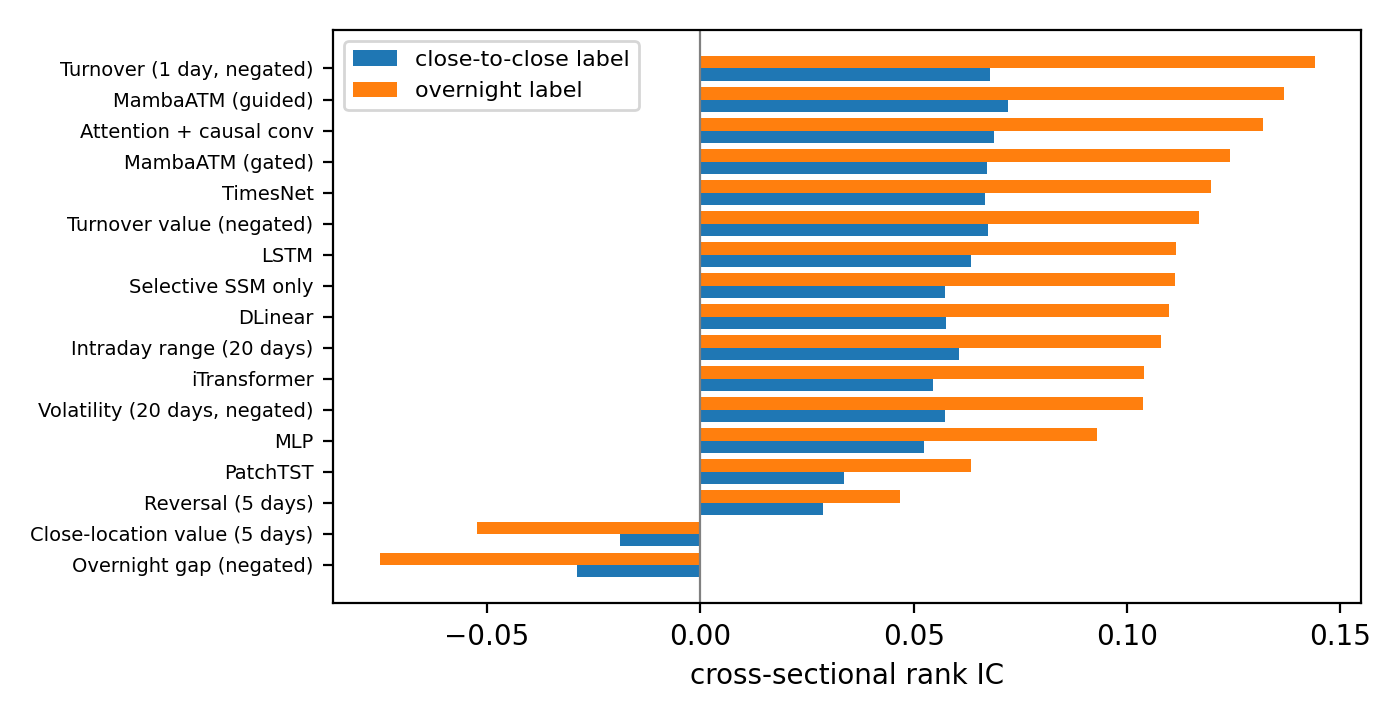
\includegraphics[width=\textwidth]{figs/ic_by_label}
	\caption{Cross-sectional rank information coefficient of each signal against the close-to-close
		label and against the overnight label. The overnight bars are systematically taller, and the
		ratio of the two is close to the ratio of the labels' standard deviations.}\label{fig:iclabel}
\end{figure}

\subsection{What the factor library already explains}
\textbf{A twenty-nine-factor library.}

Everything in this section is computed from the eight columns of the panel. The library contains
reversals over one, five and twenty days; momentum over the window; the standard deviation of returns
over twenty and sixty days, the downside-only deviation, the mean daily range and the maximum daily
return; the skewness and kurtosis of returns; the close-location value and the upper and lower shadows
of the daily bar; the turnover rate and its variability, the Amihud illiquidity ratio, the log
turnover value and a volume spike measure against its own twenty-day mean; the mean overnight and
intraday components of the stock's own returns and their volatilities; and the stock's beta to the
equal-weighted panel. Each is oriented so that the literature's prior puts the higher score on the
higher return, and each is evaluated on exactly the rows the models are evaluated on.

\textbf{Neutralisation.}

For each day the score of interest is regressed cross-sectionally on the twenty-nine factors, and the
residual is correlated with the realised return in the usual rank way. Table~\ref{tab:neutral}
reports the raw and the residual information coefficient for the ten models, on both labels; for a
factor, the factor is left out of its own regression, which is the only way the comparison is
meaningful. A handful of individual factors retain more residual overnight information than any model
does, evaluated under the same leave-one-out rule, and the next subsection reports which.

\begin{table}[!ht]
	\centering
	\caption{Raw and factor-neutralised information coefficients for the ten models. The last column is the share of the cross-sectional variance of a model's score that is linear in the twenty-nine-factor library.}
	\label{tab:neutral}
	{\scriptsize
\setlength{\tabcolsep}{2pt}
\begin{tabular}{lccccc}
\toprule
\textbf{Score} & \textbf{IC cc} & \textbf{IC night} & \textbf{Residual night} & \textbf{$t$ resid} & \textbf{$R^2$ on factors} \\
\midrule
MambaATM (gated) & 0.0671 & 0.1241 & 0.0047 & 2.7 & 0.76 \\
MambaATM (guided) & 0.0721 & 0.1369 & 0.0041 & 2.3 & 0.81 \\
Selective SSM only & 0.0574 & 0.1112 & 0.0015 & 0.8 & 0.75 \\
DLinear & 0.0576 & 0.1098 & -0.0018 & -1.0 & 0.88 \\
Attention + causal conv & 0.0688 & 0.1319 & -0.0025 & -1.4 & 0.89 \\
LSTM & 0.0633 & 0.1115 & -0.0026 & -1.4 & 0.77 \\
TimesNet & 0.0667 & 0.1197 & -0.0029 & -1.7 & 0.81 \\
PatchTST & 0.0337 & 0.0635 & -0.0057 & -3.3 & 0.69 \\
MLP & 0.0525 & 0.0929 & -0.0109 & -6.1 & 0.74 \\
iTransformer & 0.0546 & 0.1039 & -0.0139 & -7.6 & 0.79 \\
Two cheap factors & 0.0763 & 0.1475 & nan & nan & 1.00 \\
\bottomrule
\end{tabular}
}

\end{table}

Three readings matter.

\textbf{Most of a model's score is a factor combination.} Between \rSquaredLo{} and \rSquaredHi{} of the
cross-sectional variance of a model's score is linear in the library. The loading is dominated by
turnover and turnover value, since the standardised coefficient on the one-day turnover factor is
between $+0.6$ and $+0.9$ for every architecture, so the models are, to a first approximation, rediscovering
the illiquidity and low-turnover premia.

\textbf{What is left is small and barely significant.} On the close-to-close label the largest
residual coefficient among the models belongs to the proposed hybrid at \residCcBest, with the guided
variant lower; on the overnight label, where the information is, the proposed hybrid retains
\residProp{} ($t = \tResidProp$) and the guided variant \residGuided{} ($t = \tResidGuided$). Those
are positive and, for the hybrid, distinguishable from zero, but they are a fifth of the raw number
and are smaller than what a single factor keeps.

\textbf{A factor beats every model on residual information.} \bestFactorName{} retains
\bestFactorResid{} ($t = \bestFactorT$) after the other twenty-eight are controlled for, which is five
times the proposed hybrid's residual. The pattern is not a single outlier, since intraday range,
momentum, upper shadow, the five-day intraday return and the five-day overnight gap all retain more
residual overnight information than any model. The honest summary is
that these architectures add a small amount of information that the library does not contain, and less
than the library contains on its own.

\subsection{Costs, capacity and execution}
\textbf{A cost model with the parts that differ between the two sides.}

The earlier sections charge a constant rate per position change, and that is enough to establish that
the daily long-flat rule does not repay its own trading. It is not enough to price a portfolio, because
a constant rate hides which component of the cost is binding and at what size. This section charges
what a Chinese account actually pays, with the components separated so that the break-even value of
each can be read off, and it prices the long-short cross-sectional book rather than the long-flat rule
of a single name.

\begin{itemize}
	\item \textbf{Commission} of \commissionBp{} basis points per side, and a transfer fee of
	\transferBp{} basis points per side.
	\item \textbf{Stamp duty} of \stampBeforeBp{} basis points on the sell side only, falling to
	\stampAfterBp{} basis points on \stampDate, so the rate changes inside the sample.
	\item \textbf{Slippage} of \slippageBp{} basis points per side.
	\item \textbf{Square-root impact}, $\eta\,\sigma\sqrt{Q/\text{ADV}}$ with $\eta = \impactCoef$,
	the stock's daily volatility from the look-back window, $Q$ the traded notional and ADV the
	turnover value of the signal day. Impact therefore depends on the size of the book, which is what
	turns a net return into a capacity curve.
	\item \textbf{Borrow} of \borrowPct{} per cent per year on the short leg, since a long-short book
	in this market cannot be assumed to borrow for free.
	\item \textbf{Tradability}, meaning that a name which closed at or beyond a 9.8 per cent move on the
	signal day is excluded from the next day's entry, because a limit-up name cannot reliably be bought.
\end{itemize}

Turnover is charged on the change in each leg's weights, with a name's position tracked by identity
rather than by row, and a leg that is fully replaced costs two units of \mbox{sum~$|\Delta w|$}. Long-only portfolios are
evaluated by the same code with no borrow and no short leg.

\textbf{Break-even fees and capacity.}

Table~\ref{tab:realcost} reports the decomposition for each signal at daily and weekly rebalancing.
The break-even commission column is the symmetric one-way rate at which the long-short book nets zero,
and the final column is the 95th percentile of the traded notional as a fraction of the day's turnover
value, which is the number that decides whether the impact term is being extrapolated.

\begin{table}[!ht]
	\centering
	\caption{Cost decomposition of the long-short book and the book size at which it breaks even. All figures are annualised percentages except break-even size in million CNY and the 95th percentile of participation. The tradability filter removes a stock on a day when its move on the signal day reaches the price limit, the borrow fee is charged on the short leg, and the impact is evaluated at a reference book of 100 million CNY per leg, from which the other book sizes follow the square-root law.}
	\label{tab:realcost}
	{\scriptsize
\setlength{\tabcolsep}{2pt}
\begin{tabular}{lcccccc}
\toprule
\textbf{Score} & \textbf{Hold} & \textbf{Gross} & \textbf{Costs} & \textbf{Net} & \textbf{Break-even} & \textbf{$p_{95}$ part.} \\
\midrule
MambaATM (guided) & 1 & +115.3 & 217.8 & -102.4 & 16 & 39 \\
MambaATM (guided) & 5 & +68.4 & 52.1 & +16.4 & 222 & 38 \\
MambaATM (gated) & 1 & +98.7 & 222.7 & -124.0 & 7 & 33 \\
MambaATM (gated) & 5 & +54.5 & 54.0 & +0.4 & 103 & 33 \\
Attention + causal conv & 1 & +89.0 & 227.3 & -138.3 & 6 & 39 \\
Attention + causal conv & 5 & +47.2 & 55.1 & -7.9 & 62 & 39 \\
LSTM & 1 & +96.8 & 225.5 & -128.7 & 8 & 37 \\
LSTM & 5 & +60.5 & 55.1 & +5.4 & 133 & 38 \\
low\_turnover & 1 & +70.7 & 190.3 & -119.5 & 5 & 60 \\
low\_turnover & 5 & +44.0 & 47.1 & -3.1 & 81 & 60 \\
small\_amount & 1 & +59.5 & 223.2 & -163.7 & 2 & 71 \\
small\_amount & 5 & +41.7 & 53.1 & -11.4 & 50 & 71 \\
\bottomrule
\end{tabular}
}

\end{table}

At daily rebalancing the answer is unambiguous, since the proposed hybrid has a gross return of
\grossDay{} per year, fees take a third of it, and impact at \aumRefM{} million per leg takes
\impactDay, twice what is left, so the net is \netDay. The break-even book sizes are in the tens of
millions of CNY, which is not a strategy. At weekly rebalancing the same signal keeps most of its
gross return, fees fall, and impact becomes a large but survivable charge; the viable region is weekly
rebalancing on the liquid half of the panel.

\textbf{Where the money comes from, and why the close matters.}

Fig.~\ref{fig:attribution} decomposes the gross return of the weekly book
into its two legs and repeats the calculation for a book entered at the open. For the proposed hybrid
the overnight leg contributes \onWkW{} per year against a total gross of \grossWk, while the intraday
leg subtracts \idWk. Entering at the open instead of the close, which is what an investor does who
waits for the opening auction after the signal is formed, leaves \openWk, that is, essentially
nothing. The decomposition therefore explains the close-to-close result and the execution rule
together, because the signal is a prediction about the closing-to-opening gap and the position has to
exist before that gap.

\begin{figure}[H]
	\centering
	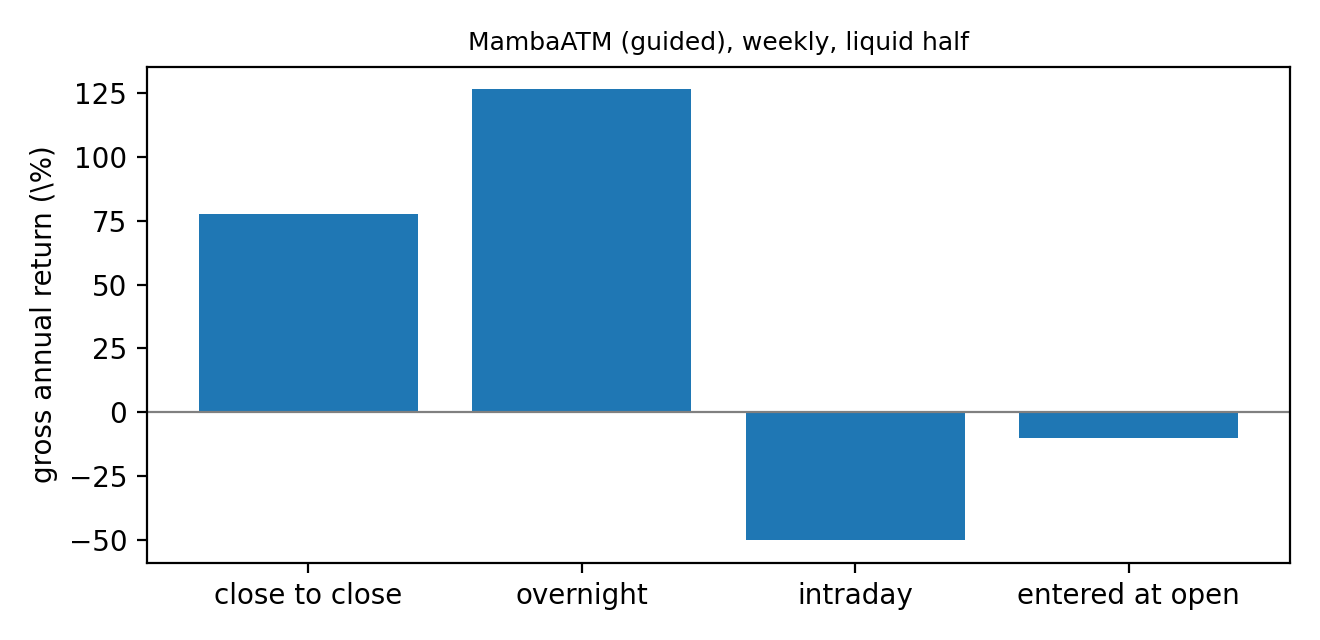
\includegraphics[width=0.80\textwidth]{figs/attribution}
	\caption{Gross annual return of the weekly long-short book on the liquid half of the panel,
		split into the close-to-close total, the overnight leg, the intraday leg, and the total that
		would remain if the book were entered at the open.}\label{fig:attribution}
\end{figure}

\textbf{Smoothing the signal does not help.}

The natural way to cut turnover without retraining is to smooth the score across days. It fails, and
the failure is informative, because the day-to-day change in a model's score is the signal rather
than noise. An
exponential moving average with a twenty-day halflife cuts the overnight coefficient from
\icOnGuided{} to \emaOn{} and turns the net return into \emaNet{} per cent per year. The only levers
that work are the holding period and the liquidity of the
universe, both of which reduce the number of trades rather than the information in each trade.

\textbf{Combining the model with cheap factors.}

The models and the factor library are not the same signal, even though the models mostly span the
library, in that the library's best member retains more residual information than any model. A
combination should therefore beat its components, and it does. Table~\ref{tab:combine} reports a scan
that standardises the model score and the average of four cheap factors within each day and mixes them
with a weight from zero, which is the factors alone, to one, which is the model alone. The best
variant puts three quarters of the weight on the factors, and it earns \combGross{} per year gross and
\combNet{} net at
\aumRefM{} million per leg, against \modNet{} for the model alone and \facNet{} for the factors alone,
with a break-even book size of \combCap{} million against \modCap{} and \facCap{}. Its overnight
information coefficient is \combIcOn{} ($t = \combTOn$), higher than either component's.

\begin{figure}[H]
	\centering
	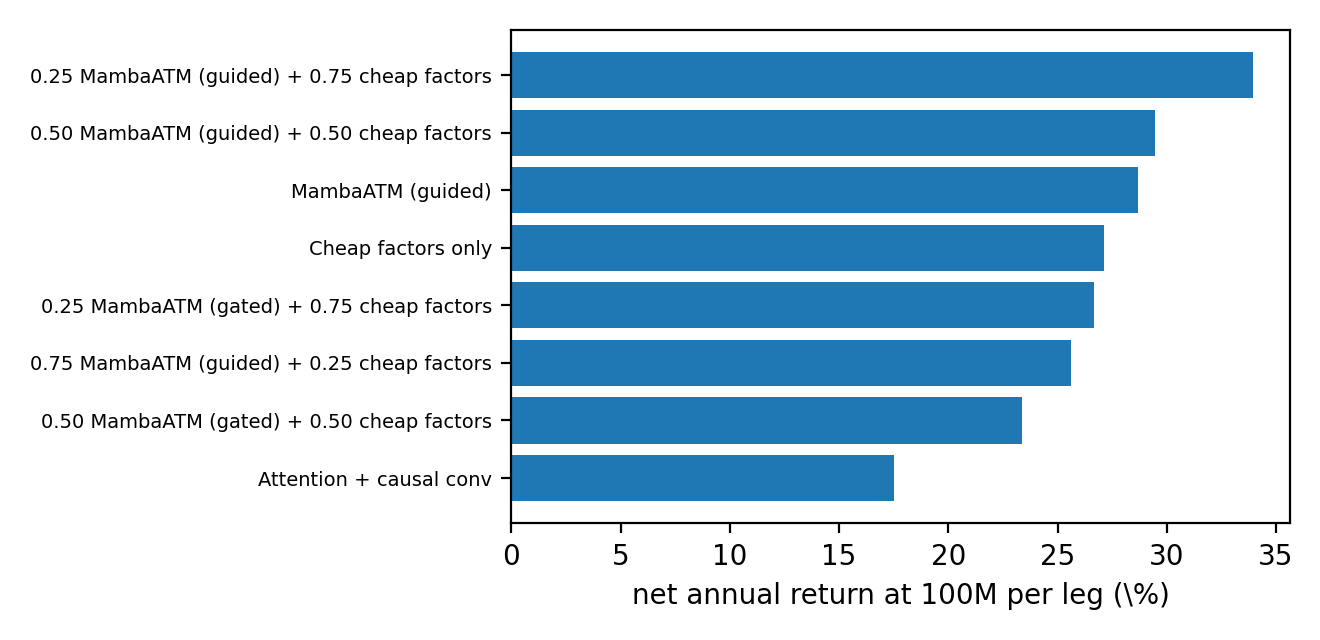
\includegraphics[width=\textwidth]{figs/combine}
	\caption{Net annual return at \aumRefM{} million per leg of the weekly book on the liquid half of
		the panel, for the model, the factor combination, and mixtures of the two. The best mixture
		places three quarters of the weight on the factors.}\label{fig:combine}
\end{figure}

\begin{table}[!ht]
	\centering
	\caption{Mixing the model score with four cheap factors, weekly on the liquid half, with the weight scanned from zero to one. Costs are the commission, transfer fee, stamp duty and slippage, the square-root impact at a reference book of 100 million CNY per leg, and the borrow fee on the short leg, so the gross return less the costs is the net return. The tradability filter of Table~\ref{tab:realcost} is applied here as well, so the two tables differ only in the universe, this one being the liquid half of the panel, and in the reference book size.}
	\label{tab:combine}
	{\scriptsize
\setlength{\tabcolsep}{2pt}
\begin{tabular}{lcccccc}
\toprule
\textbf{Signal} & \textbf{IC} & \textbf{IC night} & \textbf{Gross} & \textbf{Costs} & \textbf{Net} & \textbf{Break-even} \\
\midrule
0.25 guided + 0.75 factors & 0.087 & 0.159 & +79.1 & 45.2 & +33.9 & 526 \\
0.50 guided + 0.50 factors & 0.086 & 0.161 & +75.8 & 46.4 & +29.4 & 443 \\
MambaATM (guided) only & 0.072 & 0.137 & +77.6 & 48.9 & +28.7 & 404 \\
Four cheap factors only & 0.078 & 0.143 & +71.8 & 44.7 & +27.1 & 409 \\
0.25 gated + 0.75 factors & 0.085 & 0.156 & +72.7 & 46.0 & +26.7 & 397 \\
0.75 guided + 0.25 factors & 0.082 & 0.154 & +73.3 & 47.7 & +25.6 & 374 \\
0.50 gated + 0.50 factors & 0.085 & 0.154 & +71.1 & 47.7 & +23.4 & 343 \\
Attention + causal conv & 0.069 & 0.132 & +69.2 & 51.7 & +17.5 & 241 \\
attention+conv + EMA1 & 0.067 & 0.129 & +67.8 & 50.3 & +17.5 & 242 \\
MambaATM (gated) only & 0.067 & 0.124 & +65.6 & 48.9 & +16.8 & 254 \\
gatedfusion-guided + EMA1 & 0.072 & 0.138 & +63.8 & 47.1 & +16.7 & 254 \\
Selective SSM only & 0.057 & 0.111 & +65.1 & 48.5 & +16.5 & 247 \\
0.75 gated + 0.25 factors & 0.078 & 0.141 & +62.7 & 48.6 & +14.1 & 227 \\
dlinear + EMA5 & 0.053 & 0.110 & +61.4 & 48.0 & +13.3 & 204 \\
LSTM & 0.063 & 0.112 & +64.2 & 51.5 & +12.6 & 199 \\
lstm + EMA1 & 0.064 & 0.113 & +62.2 & 50.1 & +12.1 & 194 \\
TimesNet & 0.067 & 0.120 & +61.2 & 49.8 & +11.4 & 193 \\
dlinear + EMA1 & 0.058 & 0.113 & +62.0 & 52.2 & +9.8 & 172 \\
gatedfusion + EMA1 & 0.068 & 0.127 & +56.2 & 46.8 & +9.5 & 179 \\
timesnet + EMA1 & 0.066 & 0.119 & +49.2 & 47.9 & +1.4 & 110 \\
timesnet + EMA5 & 0.058 & 0.108 & +45.4 & 44.6 & +0.8 & 105 \\
ssm-only + EMA1 & 0.058 & 0.112 & +47.6 & 47.1 & +0.5 & 103 \\
gatedfusion-guided + EMA5 & 0.062 & 0.123 & +43.9 & 44.2 & -0.3 & 98 \\
DLinear & 0.058 & 0.110 & +52.1 & 53.2 & -1.1 & 93 \\
lstm + EMA5 & 0.059 & 0.105 & +42.0 & 46.1 & -4.1 & 74 \\
attention+conv + EMA5 & 0.059 & 0.116 & +41.3 & 48.0 & -6.6 & 62 \\
gatedfusion + EMA5 & 0.060 & 0.116 & +36.0 & 44.0 & -8.0 & 51 \\
dlinear + EMA20 & 0.039 & 0.084 & +36.6 & 45.2 & -8.6 & 52 \\
MLP & 0.052 & 0.093 & +42.1 & 52.9 & -10.8 & 44 \\
ssm-only + EMA5 & 0.051 & 0.102 & +33.2 & 44.6 & -11.4 & 37 \\
mlp + EMA1 & 0.053 & 0.096 & +36.7 & 51.8 & -15.1 & 28 \\
lstm + EMA20 & 0.044 & 0.083 & +28.1 & 44.5 & -16.4 & 21 \\
gatedfusion-guided + EMA20 & 0.046 & 0.097 & +26.3 & 43.5 & -17.2 & 17 \\
gatedfusion + EMA20 & 0.044 & 0.089 & +24.9 & 43.3 & -18.4 & 14 \\
mlp + EMA5 & 0.051 & 0.095 & +30.7 & 49.6 & -18.9 & 17 \\
timesnet + EMA20 & 0.042 & 0.083 & +19.9 & 43.4 & -23.5 & 4 \\
ssm-only + EMA20 & 0.037 & 0.079 & +17.8 & 43.9 & -26.1 & 2 \\
mlp + EMA20 & 0.041 & 0.080 & +19.1 & 48.5 & -29.4 & 1 \\
attention+conv + EMA20 & 0.043 & 0.090 & +12.4 & 46.7 & -34.3 & 0 \\
\bottomrule
\end{tabular}
}

\end{table}

\subsection{Ablation of the gate, the guidance and the two branches}\label{sec:ablation}

Table~\ref{tab:ablation} separates the components. The selective state-space branch on its own
reaches \accSSM{} accuracy with \paramSSM{} parameters; the causal attention branch with a
convolution reaches \accAtt{}; the gated fusion of the two reaches \accProp{}. The gate therefore
does not improve on its better branch, because the fused model is \nGateGain{} points below the
attention branch alone, its Sharpe is lower, and on this target the extra machinery has nothing to
add. The
guided variant of Eq.~\eqref{eq:guided} reaches \accGuided{} and has a Sharpe of
\shGuided, that is \accGuidedMinusPlain{} points of accuracy and \shGuidedMinusPlain{} of Sharpe
relative to the plain gate, with \paramGuided{} against \paramProposed{} parameters. Its equal-weight
portfolio return is indistinguishable from the plain gate.

This is the result that the earlier version of this work could not have produced, because it
described the guided mechanism and implemented the gate. Having built both, the panel does not
support the stronger claim. Two tenths of a percentage point of accuracy, against a cross-sectional
standard deviation of two points, is not an improvement; giving attention the ability to modulate the
state update neither helps nor hurts, and the extra capacity is not recovered by the extra
parameters, and Table~\ref{tab:ablation} carries the cross-stock standard deviation of the same
comparison. What the gate does
is what the earlier text said the guidance did, since it lets the model weight the two branches, and
that is what should be claimed.

\begin{table}[tbp]
	\centering
	\caption{Branches and fused variants, with the cross-stock standard deviation where the quantity is a mean over stocks.}
	\label{tab:ablation}
	{\scriptsize
\setlength{\tabcolsep}{2pt}
\begin{tabular}{lccccc}
\toprule
\textbf{Component} & \textbf{Accuracy} & \textbf{F1} & \textbf{Sharpe} & \textbf{Return} & \textbf{Parameters} \\
\midrule
Attention (causal conv) & 0.518 $\pm$ 0.019 & 0.345 & +0.18 & +26.0\% & 13\,313 \\
Selective SSM only & 0.514 $\pm$ 0.022 & 0.355 & +0.05 & +16.2\% & 1\,057 \\
MambaATM (gated fusion) & 0.516 $\pm$ 0.021 & 0.356 & +0.15 & +29.9\% & 23\,242 \\
MambaATM (guided fusion) & 0.517 $\pm$ 0.021 & 0.340 & +0.12 & +22.1\% & 25\,452 \\
\bottomrule
\end{tabular}
}

\end{table}

\subsection{Sensitivity}

Three sensitivity checks are reported. The window length is varied over $T \in \{20, 60, 120\}$ days
on a fixed 58-stock subset, because a longer window gives the state-space branch more to summarise
and the attention branch more to attend over; the panel accuracy of MambaATM moves between
\accTMin{} and \accTMax{} against a majority-class rate between \accMajTMin{} and \accMajTMax, so the
gap between the model and the reference persists at every window length. The seed is varied over
three values on the same subset, which moves its accuracy by \accSeedSd{} points, of the same order
as the gap between the models in Table~\ref{tab:main}.

The third check is the test period itself, and it is the most informative. Table~\ref{tab:sensitivity}
breaks the accuracy of each model down by year, next to the majority-class rate of the same year. The
two series move together, because in the years when most stocks rose the models look accurate and in
the years when most fell they do not, and in eight of the nine years the majority-class rate is
higher than the accuracy of every learned model, including MambaATM. The co-movement is visible in
every year. The single
exception is 2025, where the majority-class rate is at its lowest and MambaATM is a fraction above it.
That co-movement is the clearest evidence that the models are learning the drift of the sample rather
than a stable cross-sectional signal, and it explains why the accuracies in Table~\ref{tab:main}
cluster so tightly, since what is being measured is how well a model's constant tendency matches the
tide of the period rather than how well it ranks stocks.

\begin{table}[tbp]
	\centering
	\caption{Window length, seed and per-year stability. Rows are present only for the runs that were made; the per-year block reports the accuracy of the proposed model against the majority-class rate of the same year.}
	\label{tab:sensitivity}
	% window length, seed and per-year stability; rows appear only for runs that were made
{\footnotesize
\setlength{\tabcolsep}{3pt}
\begin{tabular}{lccccc}
\toprule
\textbf{Setting} & \textbf{Accuracy} & \textbf{Majority class} & \textbf{Gap} & \textbf{Sharpe} & \textbf{Return} \\
\midrule
Window $T=60$, full panel (reported) & 0.516 $\pm$ 0.021 & 0.528 & -1.26 & +0.15 & +29.9\% \\
Window $T=20$, 58-stock subset & 0.516 $\pm$ 0.019 & 0.526 & -0.95 & +0.20 & +56.4\% \\
Window $T=120$, 58-stock subset & 0.516 $\pm$ 0.017 & 0.525 & -0.93 & +0.26 & +64.9\% \\
Seed 0, 58-stock subset & 0.517 $\pm$ 0.019 & 0.526 & -0.87 & +0.27 & +63.1\% \\
Seed 7, 58-stock subset & 0.517 $\pm$ 0.014 & 0.526 & -0.84 & +0.17 & +34.4\% \\
Seed 13, 58-stock subset & 0.514 $\pm$ 0.017 & 0.526 & -1.14 & +0.25 & +41.2\% \\
\midrule
\multicolumn{6}{l}{\emph{Accuracy by test year, proposed model vs majority class}} \\
  2017 & 0.448 & 0.552 & -10.45 & -- & -- \\
  2018 & 0.488 & 0.548 & -5.94 & -- & -- \\
  2019 & 0.516 & 0.518 & -0.14 & -- & -- \\
  2020 & 0.513 & 0.530 & -1.76 & -- & -- \\
  2021 & 0.516 & 0.525 & -0.93 & -- & -- \\
  2022 & 0.517 & 0.526 & -0.86 & -- & -- \\
  2023 & 0.528 & 0.547 & -1.94 & -- & -- \\
  2024 & 0.507 & 0.523 & -1.66 & -- & -- \\
  2025 & 0.514 & 0.510 & +0.45 & -- & -- \\
\bottomrule
\end{tabular}
}

\end{table}

\subsection{Efficiency}\label{sec:efficiency}

The fused model
has \paramProposed{} trainable parameters and takes \secProposed{} seconds per stock, against
\paramMLP{} and \secMLP{} seconds for the MLP, \paramPatch{} and \secPatch{} seconds for PatchTST,
and \paramSSM{} parameters for the state-space branch alone. The fused model is therefore an order
of magnitude smaller than the two transformer baselines and about \secRatio{} times slower than the
MLP. None of these differences is an obstacle to deployment; equally, none of them is an efficiency
breakthrough. The claim that a hybrid removes the quadratic cost of attention would require the
attention branch to be absent, and it is not absent in this model.

\subsection{Discussion}\label{sec:discussion}

This paper reports two results about the same panel, and the second is what explains the first.

The first is negative, and it is worth stating what it does and does not show. It does not show that
the architecture is wrong. MambaATM is within a fraction of a point of the best model in the panel,
its equal-weight portfolio loses less than buy and hold, and its per-stock Sharpe is positive. It
shows that the margin is indistinguishable from noise, since it is not the most accurate model, it is
not the model with the best risk-adjusted return, it is significantly worse than a single linear layer
with a moving-average decomposition on both counts, and it does not reach the majority-class rate. Any
claim of the form ``the hybrid is better'' would have to be supported by an experiment that this
design does not produce.

The second is that the target, and not the architecture, decides the answer. Posing the same problem
as the cross-sectional rank of the same panel, with the same features and the same models, produces a
rank information coefficient of \icCcProp{} on the close-to-close return and \icOnProp{} on the
overnight leg, and a weekly long-short book that survives realistic costs. Nothing about the models
changed between the two experiments. What changed is that the absolute direction of one stock carries
the drift of the sample, which a constant predictor already captures, whereas the ordering within a
day does not. The overnight leg is where that ordering lives, and the identity relating the two
coefficients holds for every signal tested, so the small close-to-close numbers are the overnight
signal diluted by intraday noise rather than a weak signal.

That said, the cross-sectional result is a weak result about the architecture as well. A
twenty-nine-factor library explains \rSquaredLo{} to \rSquaredHi{} of the cross-sectional variance of
the ten models, and the residual overnight coefficient of the proposed model is \residProp{}, against
\bestFactorResid{} for the best single factor, \bestFactorName. The best configuration we found gives
the model a quarter of the weight and the cheap factors three quarters, and the daily version of the
same signal is destroyed by impact at \impactDay{} a year against a gross of \grossDay. The honest
summary of the cross-sectional study is therefore that the signal is real, that most of it is already
in the factor library, that the model adds a little at weekly frequency, and that it cannot be traded
daily at any size we could test.

The earlier version of this work reported accuracies between 0.60 and 0.85 on four unnamed stocks.
Those numbers cannot be reproduced on data that passes the integrity checks of
Section~\ref{sec:audits}, and the reason is structural rather than a matter of tuning, since on a panel
where the majority-class rate is \accMaj, where the cross-sectional dispersion of accuracy is
\accPropSd, and where the accuracy of every model tracks the majority-class rate of the year, only a
leak or a selection effect can produce a gap that large. We regard the protocol, the audits and the
panel as the contribution, and the architecture as a competitive design whose advantage over simpler
alternatives is not measurable here, on either target.

Four practical implications follow. First, a daily long-flat strategy on this panel turns over between
\turnProp{} and \turnBest{} times per day depending on the model, so a cost model is not a sensitivity
check but a first-order term, and work that reports gross returns is not reporting a strategy. Second,
the trivial references have to be in the table, because on a panel that fell over most of the test
period a majority-class rule is a genuine competitor and ``beats buy and hold'' is a lower bar than it
sounds. Third, when the difference between two architectures is smaller than the standard deviation
across assets, the experiment should be redesigned rather than tuned until the difference appears.
Fourth, the choice of target is not a detail of the experimental setup but the experiment itself, so a
study that reports a hybrid architecture on the absolute direction of one stock should also say what a
constant predictor, a single linear layer and a factor library already achieve on the same data.

The specific finding about this architecture is worth separating from the general one. The selective
state-space branch is the cheapest model in the panel at \paramSSM{} parameters, and on the absolute
target it is not distinguishable from the attention branch, from the fused model, or from a linear
map. The fusion does not fail on that target, it has nothing to add there, and when the target is
changed to the one that does carry signal the fusion is again not distinguishable from its own
branches once the factor library is accounted for.

\section{Conclusion}\label{sec6}

This paper specified, implemented and evaluated a hybrid of causal attention and a selective
state-space model for daily direction prediction on Chinese equities. The specification follows the
implementation, in that the model mixes its two branches with a learned sigmoid gate and the
attention-guided modulation of the state update is a variant that is implemented, measured and
reported separately. Evaluated on \nStocks{} A-share stocks over \nStockDays{} usable stock-days
with expanding-window walk-forward folds, a purge, train-only standardisation and four recorded
audits, the model lands in the middle of a band of ten architectures, at \accProp{} accuracy against
a majority-class rate of \accMaj and behind \accBestName{} at \accBest, with an equal-weight
portfolio return of \portAnnProp{} a year at a one-way cost of $10^{-3}$ against \portAnnBH{} for buy
and hold. The limitations are the substance of the result. No learned model in the panel reaches the
majority-class rate, and the differences between architectures are smaller than the dispersion
across assets, so the ranking should be read as a band rather than an order, and the guided variant
does not improve on the gate, so the architectural idea that motivated the earlier version of this
work is not supported by these data. Costs are charged as a constant rate per position change and
slippage is modelled as a rate rather than as a function of order size, so the net returns in
Table~\ref{tab:portfolio} are optimistic for large positions, and the panel is survivorship-screened,
because stocks whose adjusted series contain an impossible move are removed and stocks that delisted
during the sample are absent, which flatters every long-only rule including buy and hold. Changing the
target does not rescue the architecture either. On the cross-sectional rank the same models carry a
rank information coefficient of \icCcProp{} on the close-to-close return and \icOnProp{} on the
overnight leg, and a weekly long-short book on the liquid half returns \netWk{} a year net of costs,
but the twenty-nine-factor library explains \rSquaredLo{} to \rSquaredHi{} of the cross-sectional
variance of those models, the residual overnight coefficient of the proposed model is \residProp{}
against \bestFactorResid{} for the best single factor, the best configuration is three quarters cheap
factors, and the daily version of the same signal is destroyed by the square-root impact. What the
panel does support is the choice of target rather than the choice of model, and the architectural
comparison that would ordinarily be proposed next, a state-space branch with no attention at all, is
already in Table~\ref{tab:main} as the single-branch model and is indistinguishable from the fused one
on the absolute target.

\backmatter

\section*{Data availability}

The daily quotes underlying this study were retrieved through the public \texttt{baostock} interface
and screened with the rule stated in Section~\ref{sec5}, which admits adjusted prices, at least
1{,}200 usable rows and no adjusted daily move beyond 25 per cent. The processed panel that the
experiments read, one \texttt{utf-8-sig} CSV per stock with the exchange's own Chinese column
headers, is released with the paper, together with the two scripts that rebuild it from the source.
The columns are, in file order, the trading date, open, close, high, low, volume, turnover value,
the quoted close-to-close return, turnover rate and previous close. The screening can therefore be
re-run and
the eight excluded names inspected.

\section*{Code availability}

The code release contains the panel builder and the screening rule, the model implementations for
all ten models including the four baselines added in this revision, the walk-forward
pipeline, the trading simulator and its cost model, the four audit scripts of Section~\ref{sec:audits},
the statistical tests, and the scripts that generate every table, every figure and every number
quoted in the text. The release also keeps the submitted model class verbatim, so the behaviour
described in Section~\ref{sec:audits} and in Table~\ref{tab:claim} remains reproducible. The
repository address is given on the title page.

\begin{appendices}
	\section{Reproduction commands}\label{app1}

	Every number and graphic in this paper comes from the released result files, and the repository
	README maps each table and figure to the script that writes it. The chain is short. The panel
	statistics of Table~\ref{tab:panel} come from \texttt{panel\_stats.py}, and the four audits of
	Section~\ref{sec:audits} from \texttt{verify\_zoo.py}. The main experiment of
	Tables~\ref{tab:main}, \ref{tab:folds} and~\ref{tab:portfolio} is one run of
	\texttt{run\_panel.py}, which on one RTX 3060 takes about \runMinutes{} minutes for \nStocks{}
	stocks, \nModels{} models and \nFolds{} folds. The portfolio table, the statistical tests and the
	per-year accuracy are computed from the saved predictions by \texttt{portfolio.py},
	\texttt{stats\_tests.py} and \texttt{by\_year.py}, without retraining anything, and
	\texttt{emit\_numbers.py}, \texttt{make\_tables.py}, \texttt{make\_figs.py} and
	\texttt{make\_paper\_assets.py} write \texttt{numbers.tex}, the table bodies and the figures. A
	one-command smoke test, \texttt{code/smoke\_test.py}, runs the whole chain on a few stocks in about
	a minute and prints the accuracy next to the majority-class rate, so the pipeline can be confirmed
	before the full run is attempted.
\end{appendices}

\newpage
\bibliography{sn-bibliography}

\end{document}

